\section*{Lista de Símbolos}\label{lista-de-simbolos}
\addcontentsline{toc}{section}{Lista de Símbolos}

\begin{longtable}[]{@{}ll@{}}
\toprule\noalign{}
Símbolo & Descrição \\
\midrule\noalign{}
\endhead
\bottomrule\noalign{}
\endlastfoot
\(n_{coords}\) & Número de cidades (coordenadas) da instância \\
\(n_{pop}\) & Tamanho da população do Algoritmo Genético \\
\(n_{reps}\) & Número de repetições independentes por experimento \\
\(p_{\text{mut}}\) & Taxa de mutação \\
\(p_c\) & Taxa de cruzamento \\
\(k_{\text{trnmt}}\) & Tamanho do torneio na seleção \\
\(n_{2\text{-opt}}\) & Número máximo de iterações da busca local
2-opt \\
\(B_{\mathrm{H2D}}\) & Volume de dados transferidos Host-to-Device \\
\(B_{\mathrm{D2H}}\) & Volume de dados transferidos Device-to-Host \\
\(T\) & Tempo de execução \\
\(\Delta C\) & Variação de custo em um movimento local \\
\(G = (V, E)\) & Grafo composto por vértices \(V\) e arestas \(E\) \\
\(c_{ij}\) & Custo (distância) entre as cidades \(i\) e \(j\) \\
\(f(x)\) & Função de aptidão (\emph{fitness}) de uma solução \(x\) \\
\(P(t)\) & População de soluções na geração \(t\) \\
\(\kappa\) & Limite de iterações para busca local \\
\end{longtable}

\listoffigures

\listoftables

\section*{Resumo}\label{resumo}
\addcontentsline{toc}{section}{Resumo}

Este trabalho investiga o impacto de diferentes estratégias de
paralelização em Unidades de Processamento Gráfico (GPUs) no desempenho
de um algoritmo memético (Algoritmo Genético híbrido com busca local
2-opt) para o Problema do Caixeiro Viajante (TSP). Foram implementadas e
comparadas quatro variantes isoalgorítmicas: uma versão sequencial em
CPU, uma versão híbrida ingênua (transferência indivíduo a indivíduo),
uma versão híbrida otimizada (processamento em lote) e uma versão
totalmente residente em GPU. Os experimentos, conduzidos em um conjunto
de 38 instâncias da TSPLIB com até 1002 cidades, demonstram que a
estratégia de paralelização influencia drasticamente o trade-off entre
tempo de execução e qualidade da solução. A variante híbrida otimizada
obteve os menores tempos de execução (Ganho de Performance médio de 5.5x
sobre a híbrida ingênua), enquanto a variante totalmente em GPU alcançou
a melhor qualidade de solução (gap médio de 0.88\%). Os resultados
evidenciam que a minimização da transferência de dados entre CPU e GPU é
crítica para o desempenho, e que arquiteturas totalmente residentes
favorecem o refinamento das soluções em problemas de otimização
combinatória.

\textbf{Palavras-chave:} Problema do Caixeiro Viajante, Algoritmos
Genéticos, Computação em GPU, CUDA, Otimização Combinatória.

\section*{Abstract}\label{abstract}
\addcontentsline{toc}{section}{Abstract}

This work investigates the impact of different parallelization
strategies on Graphics Processing Units (GPUs) on the performance of a
memetic algorithm (Genetic Algorithm hybridized with 2-opt local search)
for the Traveling Salesman Problem (TSP). Four iso-algorithmic variants
were implemented and compared: a sequential CPU version, a naive hybrid
version (individual-by-individual transfer), an optimized hybrid version
(batch processing), and a fully GPU-resident version. Experiments
conducted on a set of 38 TSPLIB instances with up to 1002 cities
demonstrate that the parallelization strategy drastically influences the
trade-off between execution time and solution quality. The optimized
hybrid variant achieved the lowest execution times (average Ganho de
Performance of 5.5x over the naive hybrid), while the fully GPU-resident
variant achieved the best solution quality (average gap of 0.88\%). The
results highlight that minimizing data transfer between CPU and GPU is
critical for performance, and that fully resident architectures favor
solution refinement in combinatorial optimization problems.

\textbf{Keywords:} Traveling Salesman Problem, Genetic Algorithms, GPU
Computing, CUDA, Combinatorial Optimization.

\begin{itemize}
\tightlist
\item
  \hyperref[lista-de-simbolos]{Lista de Símbolos}
\item
  \hyperref[resumo]{Resumo}
\item
  \hyperref[abstract]{Abstract}
\item
  \hyperref[cap1-introducao]{Capítulo 1 -- Introdução}

  \begin{itemize}
  \tightlist
  \item
    \hyperref[sec-11-contexto-e-motivacao]{1.1 Contexto e motivação}
  \item
    \hyperref[sec-12-problema-de-pesquisa]{1.2 Problema de pesquisa}
  \item
    \hyperref[sec-13-objetivo-geral]{1.3 Objetivo geral}
  \item
    \hyperref[sec-14-objetivos-especificos]{1.4 Objetivos específicos}
  \item
    \hyperref[sec-15-justificativa]{1.5 Justificativa}
  \item
    \hyperref[sec-16-organizacao]{1.6 Organização do trabalho}
  \end{itemize}
\item
  \hyperref[cap2-revisao-bibliografica]{Capítulo 2 - Revisão
  bibliográfica}

  \begin{itemize}
  \tightlist
  \item
    \hyperref[sec-2-fundamentacao-e-revisao]{2. Fundamentação teórica e
    revisão bibliográfica}

    \begin{itemize}
    \tightlist
    \item
      \hyperref[sec-21-otimizacao-tsp]{2.1 Otimização combinatória e o
      Problema do Caixeiro Viajante}
    \item
      \hyperref[sec-22-heuristicas-tsp]{2.2 Heurísticas para o TSP}

      \begin{itemize}
      \tightlist
      \item
        \hyperref[sec-221-2opt]{2.2.1 Entendendo o algoritmo \(2\)-opt}
      \end{itemize}
    \item
      \hyperref[sec-23-algoritmos-geneticos]{2.3 Algoritmos genéticos}
    \item
      \hyperref[sec-24-heuristicas-hibridas]{2.4 Heurísticas híbridas}
    \item
      \hyperref[sec-25-algoritmos-memeticos]{2.5 Algoritmos meméticos}

      \begin{itemize}
      \tightlist
      \item
        \hyperref[sec-251-ga-2opt]{2.5.1 Algoritmo Genético + \(2\)-opt}
      \end{itemize}
    \item
      \hyperref[sec-26-gpu-metaheuristicas]{2.6 Computação em GPU e
      paralelização de meta-heurísticas}

      \begin{itemize}
      \tightlist
      \item
        \hyperref[sec-261-taxonomia-paralelizacao]{2.6.1 Taxonomia de
        paralelização segundo Crainic e Toulouse}
      \item
        \hyperref[sec-262-gpu-aplicacoes-tsp]{2.6.2 Aplicações de GPU a
        meta-heurísticas para o TSP}
      \item
        \hyperref[sec-263-cpu-vs-gpu]{2.6.3 Contraste arquitetural: CPU
        vs GPU}
      \end{itemize}
    \item
      \hyperref[sec-27-comparacao-estatistica]{2.7 Comparação
      estatística de algoritmos de otimização}

      \begin{itemize}
      \tightlist
      \item
        \hyperref[sec-271-comparacoes-pareadas]{2.7.1 Comparações
        pareadas}
      \item
        \hyperref[sec-272-comparacoes-multiplas]{2.7.2 Comparações
        múltiplas}
      \end{itemize}
    \end{itemize}
  \end{itemize}
\item
  \hyperref[cap3-materiais-metodos]{Capítulo 3 -- Materiais e Métodos}

  \begin{itemize}
  \tightlist
  \item
    \hyperref[sec-31-ambiente-framework]{3.1 Ambiente computacional e
    framework experimental}

    \begin{itemize}
    \tightlist
    \item
      \hyperref[sec-311-hardware-software]{3.1.1 Hardware e sistema
      operacional}
    \item
      \hyperref[sec-312-ambiente-software]{3.1.2 Ambiente de software}
    \item
      \hyperref[sec-313-arquitetura-framework]{3.1.3 Arquitetura do
      framework experimental}
    \end{itemize}
  \item
    \hyperref[sec-32-arquitetura-variantes]{3.2 Arquitetura do framework
    e variantes algorítmicas}

    \begin{itemize}
    \tightlist
    \item
      \hyperref[sec-321-ga-base]{3.2.1 O Algoritmo Genético Base (GA +
      2-opt)}
    \item
      \hyperref[sec-322-variantes]{3.2.2 Estratégias de Paralelização
      (As 4 Variantes)}
    \end{itemize}
  \item
    \hyperref[sec-33-selecao-instancias]{3.3 Seleção de instâncias e
    protocolo experimental}
  \item
    \hyperref[sec-34-protocolo-estatistico]{3.4 Protocolo de análise
    estatística}
  \end{itemize}
\item
  \hyperref[cap4-resultados]{Capítulo 4 -- Resultados}

  \begin{itemize}
  \tightlist
  \item
    \hyperref[sec-41-resultados-experimentais]{4.1 Resultados
    Experimentais}
  \item
    \hyperref[sec-42-analise-por-instancia]{4.2 Análise por Instância}
  \item
    \hyperref[sec-43-analise-agregada]{4.3 Análise Agregada e
    Trade-offs}
  \item
    \hyperref[sec-44-melhor-algoritmo]{4.4 Melhor Algoritmo por
    Categoria de Tamanho}
  \item
    \hyperref[sec-45-discussao-geral]{4.5 Discussão Geral}
  \end{itemize}
\end{itemize}

\section{Capítulo 1 -- Introdução}\label{cap1-introducao}

\subsection{1.1 Contexto e motivação}\label{sec-11-contexto-e-motivacao}

O Problema do Caixeiro Viajante (Traveling Salesman Problem -- TSP) é um
dos problemas mais estudados em otimização combinatória
(\citeproc{ref-cook2012pursuit}{1}). Tem esse nome devido à sua história
clássica: um vendedor precisa visitar um conjunto de cidades, passando
por cada uma exatamente uma vez, e deseja minimizar a distância total
percorrida.

O objetivo é encontrar um ciclo hamiltoniano (ciclo no qual se deve
passar por todos os vértices uma vez e retornar ao vértice original).
Apesar de sua formulação simples, o TSP é NP-difícil (classe de
problemas para os quais não se conhece algoritmo polinomial eficiente)
e, na sua formulação de decisão: ``existe um tour com custo menor ou
igual a \(B\)?'', é NP-completo: não se conhece algoritmo em tempo
polinomial que o resolva em geral, embora seja fácil verificar o custo
de uma solução candidata. Cook (\citeproc{ref-cook2012pursuit}{1})
argumenta que essa combinação de simplicidade, dificuldade teórica e
rica estrutura geométrica faz do TSP um estudo de caso central tanto
para a teoria da complexidade quanto para desenvolvimento de métodos
exatos e heurísticos.

Na prática, variantes do TSP aparecem em domínios como roteirização de
veículos, planejamento de inspeções, manufatura e testes de circuitos,
genômica e astronomia, entre outros (\citeproc{ref-cook2012pursuit}{1}).
Exemplos clássicos incluem o posicionamento e ordenamento de furos em
placas de circuito impresso, logística e problemas de mapeamento
genético. Mesmo quando modelos reais são mais complexos (com janelas de
tempo, múltiplos veículos ou restrições de capacidade), é comum validar
ideias de projeto e análise de algoritmos primeiro em instâncias
clássicas do TSP, justamente pela ampla disponibilidade de referências,
testes padronizados e de soluções ótimas conhecidas.

Paralelamente, a evolução do hardware trouxe processadores gráficos
(GPUs) como plataforma acessível para computação de alto desempenho
(HPC) (\citeproc{ref-nvidia2024cuda}{2}) e com a popularização e
acessibilidade, pesquisas nestas áreas cresceram rapidamente. Modelos de
Inteligência Artificial Generativa, por exemplo, dependem fortemente
desse tipo de hardware.

GPUs oferecem milhares de núcleos relativamente simples, organizados em
um modelo de execução massivamente paralelo, mais próximo do paradigma
SIMD/SIMT descrito por Flynn e extensões modernas
(\citeproc{ref-flynn1972taxonomy}{3}). Em troca de um controle mais
restrito nos fluxos de processo e memória, essas arquiteturas entregam
uma grande largura de banda de memória (comunicação entre CPUs e GPUs) e
uma grande taxa de operações aritméticas por segundo (FLOPs), desde que
o problema ofereça operações semelhantes que possam ser executadas em
paralelo, seja utilizando paralelismo funcional (mais complexo) ou
paralelismo de dados (mais simples). Isso torna GPUs particularmente
atrativas para tarefas como o cálculo de matrizes (ganho exponencial,
como demonstrado nesse trabalho), a avaliação de grandes populações de
soluções e a aplicação de movimentos de vizinhança independentes em
heurísticas de melhoria.

Do ponto de vista das meta-heurísticas, Crainic e Toulouse propõem uma
taxonomia de paralelização que distingue estratégias baseadas em
decomposição de dados, decomposição de domínio e múltiplas trajetórias
cooperativas (\citeproc{ref-crainic2003parallel}{4}). A discussão
detalhada dessas categorias e sua adequação a arquiteturas de GPU é
apresentada na \hyperref[sec-261-taxonomia-paralelizacao]{Seção 2.6.1}.

O projeto desta monografia foca principalmente em algoritmos do tipo 1,
explorando paralelismo de dados em vizinhanças de \(2\)-opt e na
avaliação de populações em algoritmos genéticos, em linha com estudos
recentes sobre heurísticas para TSP em GPU
(\citeproc{ref-schulz2013gpu}{5},\citeproc{ref-tsp_gpu}{6},\citeproc{ref-fujimoto2011highly}{7}).

Ainda assim, nem todo algoritmo se beneficia automaticamente de uma
migração para GPU. Inicializações de kernels, movimentação de dados
entre CPU e GPU podem anular ganhos de paralelismo, especialmente em
problemas de porte pequeno ou em implementações que realizam pouco
trabalho por inicializações de kernel
(\citeproc{ref-van2013gpu}{8},\citeproc{ref-luong2013gpu}{9}).
Limitações de memória (VRAM) devem ser cuidadosamente calculadas para
que a memória total ocupada não passe do limite do hardware. Nesses
cenários, uma comparação direta entre versões em CPU e GPU exige cuidado
extra: deve-se isolar o impacto da plataforma de execução sem confundir
o efeito com mudanças na lógica do algoritmo. Ao longo deste trabalho,
esses desafios são documentados explicitamente em estudos de caso, onde
kernels são chamados de forma não cautelosa e versões otimizadas
(Capítulos 3 e 4), bem como em notas técnicas específicas sobre
\emph{overhead} de lançamentos de kernel e padrões de redução em GPU.

Este trabalho insere-se nesse contexto, investigando como acelerar,
utilizando GPU, um Algoritmo Genético (Genetic Algorithm -- GA) híbrido
com \(2\)-opt para o TSP, de forma controlada e estatisticamente
fundamentada, usando instâncias clássicas da biblioteca TSPLIB
(\citeproc{ref-reinelt1991tsplib}{10}) e um protocolo experimental com
um número adequado de repetições \(n_{reps}\) e testes estatísticos
apropriados (detalhado no \hyperref[cap3-materiais-metodos]{Capítulo
3}). A combinação entre GA e busca local é um exemplo de algoritmo
memético amplamente estudado na literatura
(\citeproc{ref-larranaga1999genetic}{11},\citeproc{ref-goldberg1989genetic}{12}),
em que operadores evolutivos globais são complementados por heurísticas
de melhoria como \(2\)-opt (\citeproc{ref-croes1958method}{13}) ou
Lin--Kernighan (\citeproc{ref-lin1973efficient}{14}). Neste Trabalho de
Conclusão de Curso, usarei a nomenclatura em inglês para alguns termos
técnicos como ``\(2\)-opt'', ``TSPLIB'', ``GPU'', ``CPU'' e ``GA''.

\subsection{1.2 Problema de pesquisa}\label{sec-12-problema-de-pesquisa}

Muitos estudos em computação de alto desempenho comparam algoritmos em
CPU e GPU utilizando implementações que diferem não apenas na plataforma
de execução, mas também em detalhes relevantes da lógica do algoritmo
(por exemplo, operadores distintos, parâmetros diferentes ou vizinhanças
não equivalentes)
(\citeproc{ref-schulz2013gpu}{5},\citeproc{ref-van2013gpu}{8},\citeproc{ref-benaini2018genetic}{15}).
Isso torna difícil atribuir ganhos de desempenho exclusivamente ao uso
da GPU, uma vez que alterações no desenho algorítmico ou na
parametrização podem, por si só, explicar diferenças observadas. Neste
trabalho, os parâmetros e operadores são mantidos fixos entre as
variantes, e as diferenças de desempenho observadas são discutidas à luz
do protocolo experimental apresentado no {[}Capítulo 3{]}.

Neste trabalho, busquei implementar as variantes do algoritmo sob as
mesmas condições. A estrutura dos algoritmos é projetada para ser
idêntica e otimizada tanto para CPU quanto para GPU, de forma justa,
para todos os Algoritmos Genéticos e para o algoritmo de busca local
\(2\)-opt, variando apenas a forma como cada ``módulo'' estrutural do
algoritmo é executado (em CPU ou em GPU) e o grau de paralelismo
utilizado. A pergunta central pode ser formulada da seguinte forma:

\begin{quote}
\textbf{Como comparar, de forma fiel, o impacto de diferentes
estratégias de paralelização utilizando GPU no desempenho de um
algoritmo memético (GA+\(2\)-opt) para o Problema do Caixeiro Viajante?}
\end{quote}

Responder a essa pergunta exige, ao mesmo tempo, um desenho experimental
cuidadoso de hiperparâmetros e validade estatística (número
significativo de instâncias, número adequado de repetições, métricas de
qualidade e tempo). Os parâmetros básicos do GA --- como tamanho de
população \(n_{pop}\), taxa de mutação \(p_{\text{mut}}\), tamanho do
torneio \(k_{\text{trnmt}}\), número de iterações de \(2\)-opt por
indivíduo \(n_{2\text{-opt}}\) e número de repetições por combinação
algoritmo--instância \(n_{reps}\) --- são escolhidos com base em
recomendações da literatura de algoritmos evolutivos
(\citeproc{ref-eiben2015introduction}{16},\citeproc{ref-goldberg1989genetic}{12})
e em análises específicas documentadas nos relatórios técnicos do
projeto. Esses valores e sua motivação são apresentados em detalhe no
\hyperref[cap3-materiais-metodos]{Capítulo 3}.

\subsection{1.3 Objetivo geral}\label{sec-13-objetivo-geral}

O objetivo geral deste trabalho é investigar e quantificar o impacto de
diferentes estratégias de paralelização em processadores gráficos, com
foco em:

\begin{itemize}
\tightlist
\item
  \textbf{Tempo de execução}: medir e comparar o tempo requerido para
  cada variante do algoritmo memético GA+\(2\)-opt;
\item
  \textbf{Qualidade das soluções}: avaliar o custo final das rotas
  obtidas e o \emph{gap} relativo ao ótimo conhecido, validando a
  viabilidade da solução;
\item
  \textbf{Manutenção de equivalência funcional}: garantir que as quatro
  variantes (GA-CPU, GA-Híbrido-Ingênuo, GA-Híbrido-Otimizado,
  GA-FullGPU) implementem exatamente a mesma lógica algorítmica,
  diferindo apenas na plataforma de execução e no grau de paralelismo;
\item
  \textbf{Metodologia estatística padronizada}: aplicar testes de
  hipótese apropriados (testes de normalidade, pareados e rankings)
  conforme recomendações da literatura proposta por Demšar
  (\citeproc{ref-demsar2006statistical}{17});
\item
  \textbf{Alinhamento com taxonomia de paralelização}: situar as
  estratégias adotadas no contexto da taxonomia proposta por Crainic e
  Toulouse
  (\citeproc{ref-crainic2003parallel}{4},\citeproc{ref-crainic2010parallel}{18}).
\end{itemize}

\subsection{1.4 Objetivos
específicos}\label{sec-14-objetivos-especificos}

Para viabilizar o objetivo geral, definem-se os seguintes objetivos
específicos:

\begin{enumerate}
\def\labelenumi{\arabic{enumi}.}
\item
  **Implementar quatro variações
  ``isoalgorítmicas''{[}\^{}isoalgorithm-disambiguation{]} de um
  Algoritmo Genético híbrido com \(2\)-opt para o TSP, que diferem
  apenas na forma e no local de execução (CPU ou GPU):
  {[}\^{}isoalgorithm-disambiguation{]}: O termo isoalgorítmico será
  utilizado neste trabalho para refletir variantes estruturalmente
  similares em sua composição.

  \begin{itemize}
  \tightlist
  \item
    uma versão executada puramente na CPU (\textbf{GA-CPU}), em que
    todas as operações (seleção, cruzamento, mutação, \(2\)-opt e
    cálculo de custo) são executadas com NumPy, servindo como base em
    CPU para as comparações. Na prática, essa versão é utilizada como
    base principalmente para instâncias de menor porte (por exemplo, com
    \(n_{coords} \leq 100\)); para instâncias maiores, a comparação de
    tempo passa a considerar como referência a versão híbrida, conforme
    discutido no Capítulo 3.
  \item
    uma versão híbrida com \(2\)-opt executada na GPU e avaliação em CPU
    (\textbf{GA-Híbrido-Ingênuo{[}\^{}ingenuity-disambiguation{]}}), que
    inicia kernels \textbf{individualmente} para cada rota e transfere
    as soluções (ou circuitos) completos entre CPU e GPU a cada
    iteração;
  \item
    uma versão híbrida otimizada (\textbf{GA-Híbrido-Otimizado}), em que
    \(2\)-opt e o cálculo de custos são executados em GPU em lote
    (\emph{batch}), reduzindo o número de lançamentos de kernel e o
    volume de dados transferidos;
  \item
    uma versão totalmente em GPU (\textbf{GA-FullGPU}), na qual
    população, operadores genéticos, busca local e avaliação permanecem
    residentes na GPU durante toda a evolução.
  \end{itemize}

  Os nomes utilizados aqui seguem as implementações
  \texttt{GeneticAlgorithmCPU}, \texttt{GeneticAlgorithmHybridNaive},
  \texttt{GeneticAlgorithmHybridOptimized} e
  \texttt{GeneticAlgorithmFullGPU} do framework experimental, cujos
  detalhes arquiteturais são apresentados no
  \hyperref[cap3-materiais-metodos]{Capítulo 3}.
  {[}\^{}ingenuity-disambiguation{]}: Na literatura, o termo ``naive''
  (ingênuo) é frequentemente utilizado para descrever implementações
  simples que não exploram otimizações avançadas.
\item
  \textbf{Selecionar um conjunto de instâncias da TSPLIB} com diferentes
  faixas de tamanho (pequenas \(n_{coords} \leq 100\), médias
  \(100 < n_{coords} \leq 400\) e grandes \(n_{coords} > 400\)). Essa
  seleção visa demonstrar os ganhos de desempenho que podem ser
  atingidos e garantir diversidade suficiente para analisar ganhos em
  escala. A divisão de faixas adotada é inspirada em estudos prévios com
  a TSPLIB (\citeproc{ref-reinelt1991tsplib}{10}), mas levemente
  ajustada para refletir o foco deste trabalho nas instâncias pequenas,
  médias e grandes selecionadas. O ajuste consiste em adotar
  explicitamente o número de coordenadas \(n_{coords} = 100\) e
  \(n_{coords} = 400\) como limites entre as faixas, em linha com o
  limiar prático utilizado para a comparação CPU/GPU e com a
  distribuição de tamanhos das instâncias efetivamente utilizadas nos
  experimentos.
\item
  \textbf{Definir um protocolo experimental reprodutível}, incluindo
  número de repetições por instância e algoritmo, critérios de parada,
  parâmetros do GA e limites práticos impostos pela capacidade de
  memória da GPU. O desenho desse protocolo segue recomendações da
  literatura de comparação de algoritmos e de testes estatísticos
  (\citeproc{ref-demsar2006statistical}{17}) e é detalhado no
  \hyperref[cap3-materiais-metodos]{Capítulo 3}.
\item
  \textbf{Aplicar um conjunto de testes estatísticos apropriados} para
  comparação de algoritmos, incluindo testes de normalidade
  (Shapiro--Wilk), testes pareados paramétricos (teste \emph{t-pareado})
  e não paramétricos (Wilcoxon), análise de rankings em múltiplas
  instâncias (teste de Friedman com pós-teste de Nemenyi) e medidas de
  tamanho de efeito (Cohen \(d\)), conforme recomendações em
  (\citeproc{ref-demsar2006statistical}{17}) e literatura correlata de
  teste de hipóteses. A metodologia estatística completa é apresentada
  no \hyperref[cap3-materiais-metodos]{Capítulo 3}.
\item
  \textbf{Analisar os resultados obtidos}, discutindo as possíveis
  condições em que cada variante algorítmica é vantajosa --- como por
  exemplo, tamanho da instância \(n_{coords}\), relação entre custos de
  comunicação e custo computacional, acesso à memória e volume de dados
  transferidos entre CPU e GPU nas direções host-to-device (H2D ou CPU
  \(\to\) GPU) e device-to-host (D2H GPU \(\to\) CPU)
  (\citeproc{ref-nvidia2024cuda}{2}) ---, limites práticos do uso de
  GPUs para o contexto de recursos limitados (paralelismo em uma placa
  gráfica já defasada e limitada) e as implicações para o projeto de
  algoritmos de roteamento em cenários reais, seguindo as taxonomias de
  paralelização de meta-heurísticas propostas por Crainic \& Toulouse
  (\citeproc{ref-crainic2003parallel}{4},\citeproc{ref-alba2005parallel}{19})
  e de estudos de caso em problemas de roteamento utilizando GPUs
  (\citeproc{ref-schulz2013gpu}{5},\citeproc{ref-tsp_gpu}{6},\citeproc{ref-fujimoto2011highly}{7}).
\end{enumerate}

\subsection{1.5 Justificativa}\label{sec-15-justificativa}

Do ponto de vista científico, o TSP continua sendo um problema de
referência para avaliar novas ideias em heurísticas e meta-heurísticas
(\citeproc{ref-cook2012pursuit}{1}). A vasta disponibilidade de estudos,
instâncias utilizadas em larga escala e muitas soluções ótimas
conhecidas, em particular as fornecidas pela TSPLIB
(\citeproc{ref-reinelt1991tsplib}{10}), na qual o projeto se baseia,
permite medir o desempenho de diferentes algoritmos tanto em termos de
qualidade quanto em tempo de execução. Ao longo deste trabalho, será
utilizada a notação \(n_{coords}\) para o número de coordenadas
(cidades) de cada instância, \(n_{pop}\) para o tamanho da população do
GA, \(n_{reps}\) para o número de repetições por combinação
algoritmo--instância, \(T\) para tempos de execução médios e
\(B_{\mathrm{H2D}}\), \(B_{\mathrm{D2H}}\) para os volumes totais de
dados transferidos entre CPU e GPU nas direções host-to-device e
device-to-host, respectivamente. Os detalhes de como esses elementos se
relacionam com os limites de memória de cada variante são discutidos no
\hyperref[cap3-materiais-metodos]{Capítulo 3}.

No campo da computação de alto desempenho, diferentes trabalhos relatam
ganhos relevantes ao portar heurísticas de melhoria e algoritmos
evolutivos para GPU, inclusive em variantes do TSP
(\citeproc{ref-schulz2013gpu}{5},\citeproc{ref-tsp_gpu}{6},\citeproc{ref-fujimoto2011highly}{7}).
Esses resultados indicam que GPUs são um hardware promissor para esse
tipo de algoritmo, mas também evidenciam um problema recorrente: em
muitas comparações, as versões em CPU e GPU diferem não apenas na
plataforma de execução, mas também em detalhes de implementação e
parametrização, o que dificulta isolar o efeito específico da
paralelização.

Além disso, para que conclusões sobre desempenho sejam confiáveis, não
basta observar poucos experimentos isolados. É necessário adotar um
desenho experimental com múltiplas repetições, tanto para instâncias
quanto para, medidas de dispersão e testes de hipótese adequados, como
discutido na literatura de comparação de algoritmos
(\citeproc{ref-demsar2006statistical}{17}). Neste trabalho, esses
cuidados são incorporados ao experimento, de modo que as diferenças
observadas entre variantes em CPU e GPU possam ser atribuídas, com maior
segurança, às estratégias de paralelização avaliadas.

Este trabalho justifica-se por combinar três elementos que, em conjunto,
fortalecem a contribuição científica:

\begin{enumerate}
\def\labelenumi{\arabic{enumi}.}
\tightlist
\item
  \textbf{Implementação de heurísticas clássicas em GPU}
  (particularmente \(2\)-opt e operadores do AG), explorando o
  paralelismo de forma explícita.
\item
  \textbf{Comparação entre variantes funcionalmente equivalentes do
  algoritmo em CPU e GPU}, mantendo fixos operadores, parâmetros e
  critérios de parada, de modo a isolar o efeito da plataforma de
  execução. {[}\^{}small-variations{]} {[}\^{}small-variations{]}:
  Algumas variações dentro deste contexto são esperadas, mas de modo
  geral, o algoritmo segue a mesma estrutura. Sempre há a possibilidade
  de haver pequenas variações, mas o autor busca manter, ao máximo, a
  consistência entre as variantes.
\item
  \textbf{Aplicação de metodologia estatística rigorosa}, com múltiplas
  repetições por instância, testes de hipótese adequados e medidas de
  tamanho de efeito.
\end{enumerate}

Os capítulos seguintes discutem em que condições cada variante é
vantajosa, quais os limites práticos do uso de GPUs e recursos limitados
e como os resultados dialogam com estudos prévios de heurísticas em GPU.

\subsection{1.6 Organização do trabalho}\label{sec-16-organizacao}

Este texto está organizado da seguinte forma:

\begin{itemize}
\tightlist
\item
  \textbf{Capítulo 2 -- Fundamentação Teórica / Revisão Bibliográfica}:
  apresenta os conceitos básicos de otimização combinatória e do TSP,
  revisa heurísticas de construção e melhoria (com ênfase em \(2\)-opt),
  discute algoritmos genéticos e meta-heurísticas híbridas, introduz
  princípios de computação em GPU e paralelização de meta-heurísticas, e
  resume abordagens estatísticas para comparação de algoritmos.
\item
  \textbf{Capítulo 3 -- Materiais e Métodos}: descreve o ambiente
  computacional, a arquitetura do framework desenvolvido (incluindo
  abstrações de backend e estratégias isoalgorítmicas), os detalhes do
  Algoritmo Genético híbrido com \(2\)-opt nas quatro variantes
  consideradas, o conjunto de instâncias TSPLIB utilizado, os parâmetros
  experimentais e o protocolo estatístico adotado.
\item
  \textbf{Capítulo 4 -- Resultados}: apresenta os resultados numéricos
  dos experimentos, incluindo estatísticas por instância, análises
  agregadas por faixa de tamanho, medidas de ganho de performance e
  qualidade das soluções, além da interpretação dos testes estatísticos
  aplicados.
\item
  \textbf{Capítulo 5 -- Discussão}: interpreta criticamente os
  resultados à luz da literatura, discute as implicações dos achados
  para o projeto de algoritmos de roteamento em GPU e analisa limitações
  do estudo.
\item
  \textbf{Capítulo 6 -- Conclusões e Trabalhos Futuros}: sintetiza as
  principais contribuições do trabalho, responde explicitamente aos
  objetivos propostos e indica possíveis extensões, como a aplicação do
  framework a problemas de roteirização mais complexos.
\item
  Elementos pós-textuais, como referências, glossário, apêndices
  técnicos e anexos com tabelas completas de resultados, são
  apresentados ao final do documento, conforme normas da instituição.
\end{itemize}

\section{Capítulo 2 - Revisão
bibliográfica}\label{cap2-revisao-bibliografica}

\subsection{2. Fundamentação teórica e revisão
bibliográfica}\label{sec-2-fundamentacao-e-revisao}

Este capítulo apresenta conceitos teóricos e a bibliografia utilizada
para contextualizar o problema estudado e as escolhas metodológicas
adotadas. São discutidos o Problema do Caixeiro Viajante (TSP) no
contexto da otimização combinatória
(\citeproc{ref-cook2012pursuit}{1},\citeproc{ref-rosenkrantz1977analysis}{20}),
sua importância geral e exemplos de utilização. Também são apresentadas
generalizações do problema e sua relação com problemas de roteamento de
veículos e variantes correlatas
(\citeproc{ref-raff1983routing}{21},\citeproc{ref-bodin1981state}{22},\citeproc{ref-tan2021vehicle}{23}),
heurísticas e meta-heurísticas clássicas para o TSP
(\citeproc{ref-croes1958method}{13},\citeproc{ref-lin1973efficient}{14},\citeproc{ref-voudouris1999tsp}{24}),
aprofundando-se então no tópico de algoritmos genéticos e algoritmos
meméticos
(\citeproc{ref-larranaga1999genetic}{11},\citeproc{ref-goldberg1989genetic}{12}),
princípios de computação em GPU
(\citeproc{ref-nvidia2024cuda}{2},\citeproc{ref-schulz2013gpu}{5},\citeproc{ref-tsp_gpu}{6}),
taxonomias de paralelização de meta-heurísticas
(\citeproc{ref-crainic2003parallel}{4},\citeproc{ref-crainic2010parallel}{18},\citeproc{ref-alba2005parallel}{19})
e de comparação estatística de algoritmos de otimização
(\citeproc{ref-demsar2006statistical}{17}).

\subsubsection{2.1 Otimização combinatória e o Problema do Caixeiro
Viajante}\label{sec-21-otimizacao-tsp}

O TSP pode ser formulado, na versão simétrica\footnote{Na versão
  assimétrica do TSP, os custos de viagem entre pares de cidades podem
  diferir dependendo da direção (ou seja, \(c_{ij} \neq c_{ji}\)). Em
  TSPs simétricos, o custo do cálculo de distâncias pode ser
  representado por uma matriz triangular que armazena apenas uma das
  metades (superior ou inferior) sem a diagonal, o que reduz o número de
  entradas únicas de \(n^2\) para \(n(n-1)/2\).}, como um problema de
encontrar um ciclo hamiltoniano de custo mínimo --- podendo este ser a
distância percorrida, combustível gasto, ou mesmo uma combinação de
fatores. Para fins deste trabalho, o custo será também chamado de
distância --- em um grafo completo não direcionado \(G = (V, E)\), no
qual cada vértice em \(V\) representa uma cidade e cada aresta
\((i, j) \in E\) possui um custo \(c_{ij} \geq 0\) entre as cidades
\(i\) e \(j\) (\citeproc{ref-cook2012pursuit}{1}). O objetivo é
determinar uma combinação das cidades que minimize a soma total dos
custos, retornando à cidade de origem. Geralmente em aplicações práticas
assume-se que a matriz de custos é métrica e euclidiana, isto é, os
custos derivam de distâncias euclidianas entre coordenadas no plano.

Do ponto de vista da complexidade, o TSP é um problema NP-difícil em sua
forma de otimização e NP-completo em sua forma de decisão
(\citeproc{ref-cook2012pursuit}{1}). Isso significa que, em geral, não
se conhece um algoritmo em tempo polinomial que resolva instâncias
arbitrárias em grande escala. Mesmo que seja relativamente fácil
verificar o custo de uma ou várias soluções candidatas, não podemos
afirmar que esta é a solução exata em tempo polinomial. Algoritmos
modernos como \texttt{Held-Karp} (\citeproc{ref-held1962dynamic}{25})
com uma complexidade temporal \(O(n^2 2^n)\) e o algoritmo
\texttt{Concorde} (\citeproc{ref-cook2012pursuit}{1}) com uma
complexidade temporal indefinida, conseguem resolver instâncias com
milhares de cidades, mas seu tempo de execução cresce exponencialmente
(\(O(n^2 2^n)\)), o que, embora assintoticamente muito superior à força
bruta (\(O(n!)\)), ainda o torna impraticável para instâncias muito
grandes \footnote{O algoritmo Held-Karp ``troca'' a complexidade
  temporal da força bruta \(O(n!)\) por uma complexidade espacial
  \(O(n 2^n)\), tornando sua viabilidade limitada a instâncias com
  \(n_{coords} \approx 40\) cidades. Já o algoritmo Concorde, baseado em
  técnicas de ramificação e corte, é capaz de resolver instâncias com
  até 85.900 cidades, mas seu desempenho depende fortemente da estrutura
  específica da instância (\citeproc{ref-cook2012pursuit}{1}).}.

Ao longo das últimas décadas, o TSP consolidou-se também como um padrão
de avaliação empírica de algoritmos, graças à disponibilidade de
coleções de instâncias padronizadas, como a TSPLIB
(\citeproc{ref-reinelt1991tsplib}{10}). Essas coleções incluem
instâncias com diferentes tamanhos, estruturas e origens (geográficas,
sintéticas, industriais), a maioria delas com soluções ótimas conhecidas
e obtidas por métodos exatos. No presente trabalho, são utilizadas
algumas dessas instâncias como base para avaliar e comparar heurísticas
e variantes paralelas de um algoritmo memético (combinações de
algoritmos evolutivos com busca local)
(\citeproc{ref-larranaga1999genetic}{11},\citeproc{ref-fujimoto2011highly}{7}).

\subsubsection{2.2 Heurísticas para o TSP}\label{sec-22-heuristicas-tsp}

Devido à dificuldade de resolver instâncias grandes do TSP exatamente,
uma vasta literatura de heurísticas tem sido desenvolvida para produzir
boas soluções em tempos de computação aceitáveis
(\citeproc{ref-cook2012pursuit}{1}). De forma geral, heurísticas podem
ser agrupadas em dois grandes tipos: heurísticas de construção e
heurísticas de melhoria.

Heurísticas de construção produzem uma solução viável ``do zero'',
frequentemente seguindo regras simples, também conhecidas como
algoritmos gulosos, como escolher iterativamente o vizinho mais próximo
ou inserir cidades em posições que causem o menor aumento de custo.
Exemplos incluem a heurística do vizinho mais próximo (nearest neighbor
--- NN), heurísticas de inserção (insertion heuristics) e variantes
baseadas em árvores de extensão mínimas (Minimum Spanning Trees ---
MSTs), como o Algoritmo de Christofides. Embora rápidas e fáceis de
implementar, essas estratégias tendem a gerar soluções de qualidade
moderada, servindo sobretudo como ponto de partida para métodos mais
sofisticados. Resultados clássicos da literatura mostram que, em
instâncias métricas, heurísticas baseadas em MST e em Christofides podem
oferecer garantias de aproximação sobre o custo ótimo de
\(\frac{3}{2}B^*\), aspecto discutido em textos de referência em
logística e roteamento (\citeproc{ref-simchi2005logic}{26}).

Heurísticas de melhoria partem de uma solução inicial e aplicam
sucessivos movimentos locais que procuram reduzir seu custo. Entre
essas, as chamadas \(k\)-opt são particularmente influentes: um
movimento \(2\)-opt consiste em remover duas arestas de um circuito e
reconectar os segmentos resultantes, escolhendo a reconexão que produz
um circuito ainda viável e de menor comprimento
(\citeproc{ref-croes1958method}{13}). Em instâncias euclidianas é comum
interpretar o \(2\)-opt como um mecanismo para eliminar cruzamentos,
mas, genericamente, ele também pode melhorar circuitos que não
apresentam interseções evidentes, ao substituir pares de arestas por
combinações de menor custo (\citeproc{ref-croes1958method}{13}).
Movimentos \(3\)-opt e extensões mais complexas, como o algoritmo de
Lin--Kernighan, generalizam essa ideia
(\citeproc{ref-lin1973efficient}{14}). Estas e outras heurísticas de
melhoria desempenham papel central em muitos algoritmos modernos para
TSP, tanto como procedimentos isolados quanto como componentes de
meta-heurísticas, sendo utilizadas como procedimentos de busca local.

Neste trabalho, a heurística \(2\)-opt é utilizada como busca local
básica acoplada ao Algoritmo Genético, em linha com estudos que combinam
heurísticas de construção simples com procedimentos de melhoria mais
complexos para obter soluções de alta qualidade em tempo razoável
(\citeproc{ref-voudouris1999tsp}{24},\citeproc{ref-larranaga1999genetic}{11},\citeproc{ref-fujimoto2011highly}{7}).

\paragraph{\texorpdfstring{2.2.1 Entendendo o algoritmo
\(2\)-opt}{2.2.1 Entendendo o algoritmo 2-opt}}\label{sec-221-2opt}

A formulação básica de um movimento \(2\)-opt pode ser descrita da
seguinte forma (\citeproc{ref-croes1958method}{13}): dado um circuito
\(C = (v_0, v_1, \dots, v_{n-1}, v_0)\) e dois índices \(i\) e \(j\)
tais que \(0 \leq i < j < n-1\), considera-se a remoção das arestas
\((v_i, v_{i+1})\) e \((v_j, v_{j+1})\) e a inserção das arestas
\((v_i, v_j)\) e \((v_{i+1}, v_{j+1})\). A variação de custo associada
ao movimento é dada por

\[
\Delta C = \bigl(c_{i,j} + c_{i+1,j+1}\bigr)
          - \bigl(c_{i,i+1} + c_{j,j+1}\bigr),
\]

onde \(c_{i,j}\) denota o custo (ou distância) entre as cidades \(i\) e
\(j\). Um movimento \(2\)-opt é aceitável quando \(\Delta C < 0\), isto
é, quando a substituição das arestas reduz o comprimento total do
circuito (\citeproc{ref-croes1958method}{13}).

Em implementações práticas, percorrem-se pares de índices \((i,j)\) em
alguma ordem predefinida até que nenhum movimento que gere um custo
menor seja encontrado ou até que um \textbf{limite máximo de iterações}
seja atingido. O conceito de ``iteração'' no contexto de \(2\)-opt
refere-se a uma passagem completa sobre a vizinhança do circuito: em
cada iteração, examina-se um conjunto de pares \((i,j)\) e aplicam-se
todos os movimentos que reduzem o custo.

Quando determinamos ``\(\kappa=10\) iterações em \(2\)-opt'', significa
que o algoritmo realizará até 10 dessas passagens completas, parando
antes se não houver mais melhorias possíveis. Sem um limite máximo, o
algoritmo continuaria até atingir um ótimo local --- o que pode ser
custoso computacionalmente em circuitos grandes
(\citeproc{ref-lin1973efficient}{14}). No contexto de algoritmos
meméticos (\hyperref[sec-25-algoritmos-memeticos]{Seção 2.5}), o número
de iterações de \(2\)-opt por indivíduo é um parâmetro crucial que
equilibra intensidade da busca local com custo computacional: muitas
iterações podem refinar excessivamente cada solução --- o alto custo
computacional despendido segue a lei dos rendimentos decrescentes ---,
enquanto poucas podem deixar melhorias óbvias sem explorar.

De forma mais detalhada, o algoritmo \(2\)-opt clássico pode ser
descrito como um procedimento iterativo de busca local aplicada a um
único circuito. Em linhas gerais, o algoritmo segue os passos:

\begin{enumerate}
\def\labelenumi{\arabic{enumi}.}
\tightlist
\item
  Começar com um circuito viável inicial \(C\) (obtido por uma
  heurística de construção qualquer).
\item
  Definir uma ordem de varredura para pares de índices \((i,j)\) com
  \(0 \leq i < j < n-1\). No presente trabalho, utiliza-se a ordem
  lexicográfica padrão, em que para cada \(i\), varia-se \(j = i+2\) até
  \(n-1\) (a restrição \(j \geq i+2\) evita movimentos
  triviais{[}\^{}trivial{]} e garante que o segmento a ser revertido
  tenha comprimento mínimo (\citeproc{ref-croes1958method}{13})).
  {[}\^{}trivial{]}: Movimentos triviais são aqueles que não alteram
  efetivamente o circuito, como tentar reverter um segmento de \(i\) a
  \(i+1\), pois \(c_{i, i+1}=c_{i+1, i}\) é uma aresta única e sua
  reversão não muda o circuito, no caso do TSP clássico explorado neste
  documento. O mesmo não se aplica para o ATSP.
\item
  Para cada par \((i,j)\), calcular \(\Delta C\) conforme a expressão
  acima.
\item
  Se \(\Delta C < 0\), aplicar o movimento \(2\)-opt correspondente, o
  que equivale a reverter o segmento \((v_{i+1}, \dots, v_j)\) do
  circuito, obtendo um novo circuito \(C'\), e marcar que houve melhora.
\item
  Repetir o processo de varredura enquanto forem encontrados movimentos
  com \(\Delta C < 0\) (isto é, até atingir um ótimo local em relação à
  vizinhança \(2\)-opt) ou até que um número máximo de iterações seja
  alcançado.
\end{enumerate}

Em uma implementação ingênua, a vizinhança \(2\)-opt de um circuito com
\(n\) cidades possui ordem \(O(n^2)\) movimentos possíveis, o que
implica um custo potencialmente elevado quando todos os pares \((i,j)\)
são examinados de forma exaustiva. Diversas otimizações são discutidas
na literatura, como o uso de listas de vizinhança, estruturas de dados
para poda de movimentos claramente não promissores e estratégias de
parada antecipada
(\citeproc{ref-lin1973efficient}{14},\citeproc{ref-larranaga1999genetic}{11}).
No contexto desta monografia, o foco recai principalmente na forma como
esse procedimento é paralelizado e acoplado ao Algoritmo Genético, mais
do que em otimizações finas da vizinhança em CPU.

A Figura\textasciitilde{}\ref{fig:2opt-flowchart} ilustra a lógica do
algoritmo \(2\)-opt clássico: o laço externo continua enquanto houver
melhorias e o número de iterações não exceder o limite. Em cada
iteração, todos os pares \((i,j)\) são examinados; movimentos com
\(\Delta C < 0\) são aplicados imediatamente, revertendo o segmento do
circuito.

Figura\textasciitilde{}\ref{fig:2opt-flowchart}: Fluxograma do algoritmo
\(2\)-opt.

\begin{Shaded}
\begin{Highlighting}[]
\NormalTok{Input: Initial tour C, max\_iterations}
\NormalTok{Output: Optimized tour C}

\NormalTok{iteration = 0}
\NormalTok{improved = true}

\NormalTok{while improved and iteration \textless{} max\_iterations do}
\NormalTok{    improved = false}
\NormalTok{    iteration = iteration + 1}
    
\NormalTok{    for i = 0 to n{-}3 do}
\NormalTok{        for j = i+2 to n{-}1 do}
\NormalTok{            delta = dist(i, j) + dist(i+1, j+1) {-} (dist(i, i+1) + dist(j, j+1))}
            
\NormalTok{            if delta \textless{} 0 then}
\NormalTok{                Reverse segment C[i+1...j]}
\NormalTok{                improved = true}
\NormalTok{            end if}
\NormalTok{        end for}
\NormalTok{    end for}
\NormalTok{end while}

\NormalTok{return C}
\end{Highlighting}
\end{Shaded}

\subsubsection{2.3 Algoritmos
genéticos}\label{sec-23-algoritmos-geneticos}

Algoritmos Genéticos (Genetic Algorithms -- GAs) são meta-heurísticas
inspiradas em princípios de evolução biológica, nas quais uma população
de soluções candidatas é iterativamente modificada por operadores
análogos à seleção natural, recombinação e mutação
(\citeproc{ref-goldberg1989genetic}{12},\citeproc{ref-eiben2015introduction}{16}).
Na sua forma mais simples, um AG mantém uma população de indivíduos
representando soluções para o problema; em cada geração, indivíduos são
selecionados com base em uma função de aptidão (fitness), recombinados
por operadores de cruzamento e perturbados por operadores de mutação. A
nova população resultante substitui total ou parcialmente a anterior, e
o processo se repete até que um critério de parada seja satisfeito.

No contexto do TSP, é comum representar cada solução como uma permutação
das cidades, utilizar operadores de cruzamento especializados para rotas
--- como Order Crossover (OX), Partially Mapped Crossover (PMX), entre
outros --- e empregar mutações que preservem a viabilidade da
permutação, como trocas de posição entre duas cidades
(\citeproc{ref-larranaga1999genetic}{11}). Estudos clássicos mostram que
GAs podem produzir soluções competitivas para o TSP quando combinados
com operadores e parâmetros adequados
(\citeproc{ref-goldberg1989genetic}{12}).

Do ponto de vista formal, um GA opera sobre uma população
\(P(t) = \{x_1^{(t)}, x_2^{(t)}, \dots, x_{n_{pop}}^{(t)}\}\) de
indivíduos (soluções candidatas) na geração \(t\). Cada indivíduo
\(x_i\) possui um valor de aptidão (\emph{fitness}) \(f(x_i)\) que mede
a qualidade da solução; no caso do TSP, \(f(x_i)\) corresponde ao custo
do circuito representado por \(x_i\), e busca-se minimizar esse valor. A
cada geração, o GA aplica três operadores principais
(\citeproc{ref-goldberg1989genetic}{12},\citeproc{ref-eiben2015introduction}{16}):

\begin{enumerate}
\def\labelenumi{\arabic{enumi}.}
\item
  \textbf{Seleção}: escolhe indivíduos de \(P(t)\) com probabilidade
  proporcional (ou baseada em ranking/torneio) à sua aptidão,
  favorecendo soluções de melhor qualidade. Formalmente, a probabilidade
  de selecionar \(x_i\) pode ser dada por
  \(p_i = f(x_i) / \sum_{j=1}^{n_{pop}} f(x_j)\) (seleção proporcional)
  ou por esquemas de torneio, nos quais um subconjunto aleatório de
  indivíduos compete e o melhor é escolhido.
\item
  \textbf{Cruzamento (recombinação)}: combina pares de indivíduos
  selecionados (``pais'') para produzir descendentes. No TSP, operadores
  como OX e PMX preservam a viabilidade das permutações, herdando
  subsequências de um dos pais e preenchendo as posições restantes com a
  ordem do outro (\citeproc{ref-larranaga1999genetic}{11}). A taxa de
  cruzamento \(p_c\) controla a fração de pares submetidos a esse
  operador.
\item
  \textbf{Mutação}: introduz pequenas perturbações aleatórias em
  indivíduos, mantendo diversidade na população. No TSP, mutações
  típicas incluem troca de duas cidades ou reversão de segmentos. A taxa
  de mutação \(p_{\text{mut}}\) controla a probabilidade de cada
  indivíduo sofrer mutação.
\end{enumerate}

Após aplicar esses operadores, forma-se a nova população \(P(t+1)\) por
meio de um esquema de substituição (geracional, com elitismo,
steady-state, etc.). A Figura\textasciitilde{}\ref{fig:ga-flowchart}
ilustra o fluxo geral de um GA
(\citeproc{ref-goldberg1989genetic}{12},\citeproc{ref-eiben2015introduction}{16}):
a população evolui iterativamente por meio de seleção (escolha de pais
com base em aptidão), cruzamento (combinação de pares de pais gerando
descendentes), e mutação (perturbações para diversidade), até que um
critério de parada seja atingido.

\begin{Shaded}
\begin{Highlighting}[]
\NormalTok{BEGIN AGA}
\NormalTok{   Make initial population at random.}
\NormalTok{   WHILE NOT stop DO}
\NormalTok{      BEGIN}
\NormalTok{         Select parents from the population.}
\NormalTok{         Produce children from the selected parents.}
\NormalTok{         Mutate the individuals.}
\NormalTok{         Extend the population adding the children to it.}
\NormalTok{         Reduce the extended population.}
\NormalTok{      END}
\NormalTok{   Output the best individual found.}
\NormalTok{END AGA}
\end{Highlighting}
\end{Shaded}

Figura\textasciitilde{}\ref{fig:ga-flowchart}: Fluxograma de Algoritmo
Genético.

\begin{Shaded}
\begin{Highlighting}[]
\NormalTok{Input: Population size N, mutation rate p\_mut, crossover rate p\_cross}
\NormalTok{Output: Best solution found}

\NormalTok{Initialize population P(0) randomly}
\NormalTok{Evaluate fitness of all individuals in P(0)}
\NormalTok{t = 0}

\NormalTok{while not stop\_condition do}
\NormalTok{    P\_new = \{\}}
    
\NormalTok{    // Elitism: keep best individuals}
\NormalTok{    Add best of P(t) to P\_new}
    
\NormalTok{    while size(P\_new) \textless{} N do}
\NormalTok{        // Selection}
\NormalTok{        parent1 = TournamentSelection(P(t))}
\NormalTok{        parent2 = TournamentSelection(P(t))}
        
\NormalTok{        // Crossover}
\NormalTok{        if random() \textless{} p\_cross then}
\NormalTok{            child = OrderCrossover(parent1, parent2)}
\NormalTok{        else}
\NormalTok{            child = parent1}
\NormalTok{        end if}
        
\NormalTok{        // Mutation}
\NormalTok{        if random() \textless{} p\_mut then}
\NormalTok{            SwapMutation(child)}
\NormalTok{        end if}
        
\NormalTok{        Add child to P\_new}
\NormalTok{    end while}
    
\NormalTok{    P(t+1) = P\_new}
\NormalTok{    Evaluate fitness of P(t+1)}
\NormalTok{    t = t + 1}
\NormalTok{end while}

\NormalTok{return Best of P(t)}
\end{Highlighting}
\end{Shaded}

\subsubsection{2.4 Heurísticas
híbridas}\label{sec-24-heuristicas-hibridas}

De forma ampla, heurísticas híbridas combinam duas ou mais estratégias
de busca, procurando explorar sinergias entre métodos com forças
complementares. No contexto de problemas de roteamento e, em particular,
do TSP, é comum combinar heurísticas de construção (como vizinho mais
próximo, inserções ou heurísticas baseadas em MST) com heurísticas de
melhoria (como movimentos \(k\)-opt) ou com meta-heurísticas
populacionais (como GAs), de modo que uma componente forneça boas
soluções iniciais e outra detalhe a exploração de vizinhanças
(\citeproc{ref-voudouris1999tsp}{24}).

Diversos autores classificam heurísticas híbridas em categorias como:
(i) \textbf{hibridização em nível de solução}, na qual uma
meta-heurística utiliza sistematicamente uma busca local (ou outro
procedimento) para melhorar indivíduos candidatos; (ii)
\textbf{hibridização em nível de algoritmo}, em que diferentes técnicas
(por exemplo, um método exato e um heurístico) são combinadas em fases
distintas ou em esquemas de cooperação; e (iii) \textbf{hibridizações
multiestágio}, nas quais diferentes heurísticas atuam em momentos
distintos do processo de resolução (inicialização, intensificação,
diversificação, etc.)
(\citeproc{ref-larranaga1999genetic}{11},\citeproc{ref-voudouris1999tsp}{24}).
Essas categorias ajudam a organizar o espectro de abordagens híbridas
reportadas na literatura, embora nem sempre haja consenso absoluto sobre
as fronteiras entre elas.

Uma extensão importante dessa ideia é o conceito de algoritmos
meméticos, nos quais operadores evolutivos (seleção, cruzamento,
mutação) são combinados com heurísticas de busca local aplicadas a
indivíduos da população, de forma sistemática
(\citeproc{ref-larranaga1999genetic}{11}). Em problemas de roteamento,
isso resulta em esquemas GA+LS, nos quais um GA guia a exploração global
do espaço de soluções e um procedimento de melhoria, como \(2\)-opt ou
Lin--Kernighan, refina soluções promissoras. Esses algoritmos tendem a
oferecer melhor equilíbrio entre exploração e intensificação do que GAs
``puros'', ao custo de maior tempo computacional por iteração.

Trabalhos como o de Fujimoto e Tsutsui
(\citeproc{ref-fujimoto2011highly}{7}) exploram justamente essa
combinação GA+busca local para o TSP em ambientes de computação
paralela, motivando a adoção de uma abordagem semelhante neste estudo. A
\hyperref[sec-25-algoritmos-memeticos]{próxima subseção} aprofunda o
conceito de algoritmos meméticos e a \hyperref[sec-251-ga-2opt]{subseção
2.5.1} descreve, em linhas gerais, o esquema GA+\(2\)-opt adotado nesta
monografia.

\subsubsection{2.5 Algoritmos
meméticos}\label{sec-25-algoritmos-memeticos}

Algoritmos meméticos podem ser vistos como uma família de
meta-heurísticas evolutivas que incorporam, explicitamente, operadores
de busca local ao ciclo de evolução populacional
(\citeproc{ref-larranaga1999genetic}{11}). A metáfora usual associa o
termo ``meme'' a unidades de informação que se propagam e se
transformam, de modo análogo a genes, mas em um nível mais alto de
organização: além da recombinação e mutação de indivíduos, há um
processo de ``aprendizado'' local que modifica soluções de forma
dirigida.

Em um algoritmo memético típico, a cada geração, parte dos indivíduos
(por exemplo, os mais aptos ou uma amostra da população) é submetida a
uma busca local, que pode ser uma heurística de melhoria como \(2\)-opt,
\(3\)-opt ou Lin--Kernighan no caso do TSP. Esse procedimento permite
refinar soluções já boas, acelerando a convergência em direção a ótimos
locais de alta qualidade. O GA fornece a diversidade global por meio de
operadores de cruzamento e mutação, enquanto a busca local intensifica a
exploração em torno de regiões promissoras do espaço de soluções.

O desenho de um algoritmo memético envolve decisões importantes, como:
(i) \textbf{quais indivíduos} serão submetidos à busca local (apenas a
elite, um subconjunto aleatório, toda a população); (ii) \textbf{com que
frequência} a busca local será aplicada (toda geração, gerações
alternadas, fases específicas do processo); e (iii) \textbf{com que
intensidade} cada chamada de busca local será executada (por exemplo,
número máximo de iterações de \(2\)-opt). Essas escolhas impactam o
balanço entre qualidade das soluções e custo computacional, bem como a
diversidade mantida na população.

Estudos fundamentais, como o de Larrañaga et al., indicam que os
algoritmos meméticos são extremamente eficientes para o Problema do
Caixeiro Viajante (TSP). Estes métodos funcionam melhor quando combinam
o cruzamento de rotas com técnicas de melhoria intensiva. Neste
trabalho, utilizamos um \textbf{Algoritmo Genético adaptado para rotas},
que possui as seguintes características:

\begin{enumerate}
\def\labelenumi{\arabic{enumi}.}
\tightlist
\item
  \textbf{Representação Numérica:} Cada solução é um circuito \(C\)
  denotando uma sequência de números inteiros representando a ordem das
  cidades.
\item
  \textbf{Seleção por Torneio:} Os ``pais'' são escolhidos através de
  competições diretas entre pequenos grupos de indivíduos.
\item
  \textbf{Cruzamento Ordenado (OX):} Um operador que preserva a ordem
  relativa das cidades herdadas dos pais.
\item
  \textbf{Mutação por Troca:} Pequenas alterações feitas trocando duas
  cidades de posição na rota.
\item
  \textbf{Substituição com Elitismo:} A nova geração substitui a antiga,
  mas preserva obrigatoriamente as melhores soluções encontradas até o
  momento.
\item
  \textbf{Hibridização:} Após essas etapas, aplica-se uma rotina de
  busca local (\(2\)-opt) para refinar os resultados.
\end{enumerate}

A viabilidade de acelerar esse processo usando placas de vídeo (GPU) foi
comprovada por Fujimoto e Tsutsui. Eles implementaram este algoritmo em
uma GPU (modelo GTX285) utilizando técnicas eficientes de soma paralela
para gerenciar os dados. Ao comparar o desempenho contra um processador
tradicional operando com \textbf{apenas um núcleo} (\emph{single-core}),
observaram que a GPU foi até \textbf{24,2 vezes mais rápida} na
instância \texttt{ts225}. Embora a comparação tenha sido feita contra um
processador mais antigo, o resultado prova que problemas de tamanho
médio (200-300 cidades) conseguem tirar proveito do paralelismo massivo
da GPU.

O processo formal de refinamento segue a lógica abaixo:

\begin{enumerate}
\def\labelenumi{\arabic{enumi}.}
\tightlist
\item
  Considere uma população inicial \(P(t)\).
\item
  Aplique os operadores genéticos (cruzamento e mutação) para criar
  descendentes.
\item
  Execute a função de \textbf{Busca Local Truncada}, denotada por
  \(\mathcal{L}(x, \kappa)\).
\item
  Esta função aplica melhorias na rota (\(2\)-opt) repetidamente até
  que:

  \begin{itemize}
  \tightlist
  \item
    A rota não possa mais ser melhorada (ótimo local); \textbf{OU}
  \item
    O número máximo de varreduras (\(\kappa\)) seja atingido.
  \end{itemize}
\item
  O parâmetro \(\kappa\) serve como um ``freio'': ele limita o tempo
  gasto refinando cada solução para evitar que o algoritmo fique lento
  demais, garantindo um equilíbrio entre qualidade e velocidade,
  mantendo a eficiência do algoritmo.
\end{enumerate}

\paragraph{\texorpdfstring{2.5.1 Algoritmo Genético +
\(2\)-opt}{2.5.1 Algoritmo Genético + 2-opt}}\label{sec-251-ga-2opt}

O esquema GA+\(2\)-opt adotado neste trabalho segue a linha de
algoritmos meméticos padrões para o TSP
(\citeproc{ref-larranaga1999genetic}{11}), nos quais um Algoritmo
Genético opera sobre uma população de permutações de cidades e, em
momentos específicos do ciclo evolutivo, aplica-se uma rotina de busca
local \(2\)-opt a alguns indivíduos. Em alto nível, cada iteração
(geração) do algoritmo pode ser descrita pelos seguintes passos:

\begin{enumerate}
\def\labelenumi{\arabic{enumi}.}
\tightlist
\item
  \textbf{Inicialização (\(t=0\))}: gerar uma população inicial \(P(0)\)
  de rotas, por exemplo, a partir de permutações aleatórias ou de
  heurísticas de construção simples (vizinho mais próximo, inserções).
\item
  \textbf{Avaliação (\emph{fitness})}: calcular o custo (comprimento)
  \(f(x_i)\) de cada rota \(x_i \in P(t)\), que servirá como medida de
  aptidão.
\item
  \textbf{Seleção}: escolher indivíduos para reprodução com base em seus
  valores de aptidão, utilizando seleção por torneio de tamanho
  \(k_{\text{trnmt}}\), favorecendo soluções de menor custo.
\item
  \textbf{Cruzamento}: combinar pares de indivíduos selecionados por
  meio de Order Crossover (OX), produzindo descendentes que preservam a
  estrutura de permutação e herdam subsequências de ambos os pais.
\item
  \textbf{Mutação}: aplicar perturbações leves às rotas (trocas de
  posição de cidades, com taxa \(p_{\text{mut}}\)) para manter
  diversidade genética.
\item
  \textbf{Busca local \(2\)-opt}: para cada descendente (ou um
  subconjunto, conforme a estratégia), aplicar
  \(\mathcal{L}(x, n_{2\text{-opt}})\) --- isto é, executar até
  \(n_{2\text{-opt}}\) iterações de \(2\)-opt --- de modo a refinar
  localmente as rotas resultantes. Esta etapa é o que transforma o GA em
  um algoritmo memético, introduzindo intensificação explícita da busca.
\item
  \textbf{Substituição}: formar a nova população \(P(t+1)\) combinando
  os melhores indivíduos de \(P(t)\) (elitismo) com os descendentes
  refinados, garantindo que as melhores soluções sejam preservadas ao
  longo das gerações.
\end{enumerate}

O processo repete-se até que um critério de parada seja satisfeito
(número máximo de gerações, estagnação da aptidão ou atingimento do
custo ótimo conhecido). A
Figura\textasciitilde{}\ref{fig:ga2opt-flowchart} ilustra o fluxo
completo do GA+\(2\)-opt memético
(\citeproc{ref-larranaga1999genetic}{11}): a busca local de \(2\)-opt
(etapa destacada) é aplicada após os operadores genéticos (seleção por
torneio, cruzamento OX, mutação swap), refinando cada descendente com
até \(n_{2\text{-opt}}\) iterações de \(2\)-opt
(\(\mathcal{L}(x, n_{2\text{-opt}})\)) antes da formação da nova
população. Esse acoplamento caracteriza o algoritmo como memético,
combinando exploração global (GA) e intensificação local (\(2\)-opt).

Figura\textasciitilde{}\ref{fig:ga2opt-flowchart}: Fluxograma do
algoritmo GA+\(2\)-opt.

No contexto deste trabalho, essa etapa de busca local será
posteriormente mapeada para diferentes implementações em CPU e GPU
(GA-CPU, GA-Híbrido-Ingênuo, GA-Híbrido-Otimizado, GA-FullGPU), mantendo
a mesma lógica de aplicação de \(2\)-opt (mesma vizinhança, mesmos
limites de iterações \(n_{2\text{-opt}}\)), de forma a preservar o
caráter estruturalmente equivalente das variantes. Os detalhes
operacionais, incluindo a forma precisa de parametrizar
\(n_{2\text{-opt}}\), \(n_{pop}\), \(p_{\text{mut}}\) e os critérios de
parada do GA, são apresentados no
\hyperref[cap3-materiais-metodos]{Capítulo 3}.

\subsubsection{2.6 Computação em GPU e paralelização de
meta-heurísticas}\label{sec-26-gpu-metaheuristicas}

Processadores gráficos (GPUs) evoluíram, nas últimas décadas, de
dispositivos voltados principalmente para renderização gráfica para
plataformas de computação de uso geral (GPGPU - General-purpose
computing on GPUs), amplamente utilizadas em aplicações científicas e de
inteligência artificial (\citeproc{ref-nvidia2024cuda}{2}). O modelo de
programação CUDA, por exemplo, organiza o trabalho em grades
(\emph{grids}) de blocos de threads, seguindo um paradigma de execução
massivamente paralelo próximo ao SIMT (Single Instruction, Multiple
Threads), relacionado às classificações de arquiteturas de Flynn
(\citeproc{ref-flynn1972taxonomy}{3}). Nessa configuração, milhares de
threads executam o mesmo kernel sobre dados distintos, o que é adequado
a tarefas com alto grau de paralelismo em dados.

Internamente, as threads em uma GPU são agrupadas em \emph{warps}
(tipicamente 32 threads em arquiteturas NVIDIA), que executam a mesma
instrução simultaneamente (SIMT - \emph{Single Instruction, Multiple
Threads}) (\citeproc{ref-nvidia2024cuda}{2}). Isso difere do modelo SIMD
(\emph{Single Instruction, Multiple Data}) tradicional de CPUs, onde uma
única instrução opera sobre vetores de dados, pois no SIMT cada thread
possui seu próprio contador de programa e estado de registradores,
permitindo maior flexibilidade, embora a divergência de fluxo dentro de
um warp possa penalizar o desempenho. Segundo a taxonomia de Flynn
(\citeproc{ref-flynn1972taxonomy}{3}), conforme introduzido na
\hyperref[sec-11-contexto-e-motivacao]{Seção 1.1}, enquanto CPUs
modernas operam predominantemente no modelo MIMD (\emph{Multiple
Instruction, Multiple Data}) com extensões SIMD \footnote{Embora CPUs
  sejam classificadas como MIMD (Multiple Instruction, Multiple Data),
  processadores modernos incorporam extensões vetoriais (SIMD) como AVX
  e SSE para acelerar operações em dados contíguos. Isso cria um modelo
  híbrido onde múltiplos fluxos de execução independentes (threads)
  podem, individualmente, explorar paralelismo de dados em nível de
  instrução.}, as GPUs maximizam o \emph{throughput} dedicando
transistores para processamento massivo de dados (SIMD/SIMT) em
detrimento de caches grandes e controle de fluxo, sendo ideais para
cargas de trabalho onde a mesma operação é aplicada a grandes volumes de
dados independentes.

\paragraph{2.6.1 Taxonomia de paralelização segundo Crainic e
Toulouse}\label{sec-261-taxonomia-paralelizacao}

A taxonomia de Crainic e Toulouse
(\citeproc{ref-crainic2003parallel}{4},\citeproc{ref-crainic2010parallel}{18})
classifica as estratégias de paralelização de meta-heurísticas em três
categorias principais, cada uma com adequação distinta a arquiteturas de
hardware:

\begin{enumerate}
\def\labelenumi{\arabic{enumi}.}
\tightlist
\item
  \textbf{Tipo 1: Paralelismo de Baixo Nível (Decomposição de Dados)}

  \begin{itemize}
  \tightlist
  \item
    \textbf{Descrição:} O foco é na paralelização de tarefas
    computacionalmente intensivas dentro de uma iteração da
    meta-heurística, como a avaliação da função objetivo ou a exploração
    de vizinhança. O fluxo de controle do algoritmo permanece
    centralizado.
  \item
    \textbf{Adequação:} Ideal para arquiteturas \textbf{SIMD/SIMT
    (GPUs)}. Como a mesma operação (ex: cálculo de distância) é aplicada
    a muitos dados (ex: rotas, cálculos de matrizes), o \emph{overhead}
    de inicializações de kernels e transferência é mínimo e o
    \emph{throughput} é maximizado.
  \item
    \textbf{Exemplo Real:} Rocki e Suda (\citeproc{ref-tsp_gpu}{6})
    utilizam paralelismo Tipo 1 para avaliar movimentos \(2\)-opt em
    paralelo na GPU. Cada thread calcula o ganho de uma troca de
    arestas, permitindo explorar vizinhanças massivas em tempo reduzido.
  \end{itemize}
\item
  \textbf{Tipo 2: Decomposição do Domínio}

  \begin{itemize}
  \tightlist
  \item
    \textbf{Descrição:} O espaço de busca ou as variáveis de decisão são
    particionados em subconjuntos (técnica comum em VRPs no geral), e a
    meta-heurística opera em paralelo sobre essas partições.
  \item
    \textbf{Adequação:} Mais apropriado para arquiteturas \textbf{MIMD
    (Clusters ou CPUs Multicore)}. Subproblemas distintos podem ter
    tempos de convergência variados, o que causa divergência de execução
    em uma GPU (onde as 32 threads de cada warp devem ser
    sincronizadas).
  \item
    \textbf{Exemplo Real:} Em problemas de Roteamento de Veículos com
    Múltiplos Depósitos (MDVRP), Diversos autores
    (\citeproc{ref-simchi2005logic}{26}) descrevem estratégias onde cada
    ``depósito'' é otimizado por um processo independente em uma CPU,
    com trocas ocasionais de clientes entre depósitos.
  \end{itemize}
\item
  \textbf{Tipo 3: Múltiplas Trajetórias (Buscas Independentes ou
  Cooperativas)}

  \begin{itemize}
  \tightlist
  \item
    \textbf{Descrição:} Múltiplas instâncias da meta-heurística (ou
    meta-heurísticas diferentes) exploram o espaço de soluções
    simultaneamente. Podem ser independentes (\emph{multi-start}) ou
    cooperativas (troca de informações).
  \item
    \textbf{Adequação:} Versátil. Funciona bem em:

    \begin{itemize}
    \tightlist
    \item
      \textbf{Clusters/CPUs} para algoritmos complexos e heterogêneos,
      através de técnicas de \texttt{multithreading} e
      \texttt{multiprocessing}, por exemplo.
    \item
      \textbf{GPUs} para muitas execuções de algoritmos leves e
      idênticos, como \emph{Island Models}.
    \item
      \textbf{Combinados}: Processamento massivamente paralelo, conforme
      revisado por Schulz et al. (\citeproc{ref-schulz2013gpu}{5}).
    \end{itemize}
  \item
    \textbf{Exemplo Real:} Luong et al. (\citeproc{ref-luong2013gpu}{9})
    implementam um modelo de ilhas em GPU, onde milhares de pequenas
    populações evoluem em paralelo (cada uma em um bloco de threads),
    trocando periodicamente seus melhores indivíduos via memória
    compartilhada.
  \end{itemize}
\end{enumerate}

De forma resumida, a Figura\textasciitilde{}\ref{fig:crainic-taxonomy}
coloca lado a lado esses três tipos: a partir de uma meta-heurística
sequencial, pode-se paralelizar apenas a avaliação de
vizinhança/população (Tipo 1), decompor o conjunto de variáveis em
subproblemas (Tipo 2) ou rodar várias buscas completas em paralelo,
independentes ou cooperativas (Tipo 3).

Figura\textasciitilde{}\ref{fig:crainic-taxonomy}: Resumo dos três tipos
de paralelização de Crainic e Toulouse.

No contexto deste trabalho, as variantes desenvolvidas enquadram-se
predominantemente no \textbf{Tipo 1}, focando na aceleração da avaliação
de vizinhança \(2\)-opt e operadores genéticos via paralelismo de dados
massivo na GPU.

\paragraph{2.6.2 Aplicações de GPU a meta-heurísticas para o
TSP}\label{sec-262-gpu-aplicacoes-tsp}

Aplicações de GPU a meta-heurísticas para o TSP exploram principalmente
paralelismo em dados, seja na avaliação em massa de rotas em algoritmos
genéticos (por exemplo, via cálculos de redução em GPU), seja aplicando
paralelismo a movimentos de vizinhança em heurísticas de melhoria
(\citeproc{ref-schulz2013gpu}{5},\citeproc{ref-tsp_gpu}{6},\citeproc{ref-fujimoto2011highly}{7}).
Outros trabalhos investigam paralelização de Recozimento Simulado,
Colônias de Formigas (ACO) e outras meta-heurísticas em GPU, geralmente
aproveitando o grande número de threads para explorar múltiplas soluções
ou vizinhanças em cada passo da busca
(\citeproc{ref-binjubier2024gpu}{27},\citeproc{ref-rey2018cpu}{28},\citeproc{ref-abdelatti2020improvedgpuheuristic}{29}).
Esses estudos motivam o uso de GPUs como plataforma para acelerar
algoritmos meméticos, mas também evidenciam desafios relacionados à
movimentação de dados entre CPU e GPU, à escolha de granularidade
adequada de kernels, à ocupação dos multiprocessadores e às limitações
de memória (VRAM). Esses aspectos são retomados no
\hyperref[cap3-materiais-metodos]{Capítulo 3}, ao descrever o desenho
dos kernels de \(2\)-opt e as estratégias de controle de memória
adotadas neste trabalho.

\paragraph{2.6.3 Contraste arquitetural: CPU vs
GPU}\label{sec-263-cpu-vs-gpu}

As figuras \ref{fig:cpu-gpu-contrast}, \ref{fig:cpu-gpu-detail} e
\ref{fig:gpu-internal} ajudam a visualizar, de forma simples, como CPUs
e GPUs foram pensadas para resolver problemas diferentes. De maneira
geral, CPUs têm poucos núcleos mais complexos e flexíveis. Uma parte
grande da área do chip é usada para controle de fluxo, previsão de
desvios e vários níveis de cache, o que favorece programas sequenciais,
com muitas decisões e acesso irregular à memória. Nas GPUs acontece o
contrário: a maior parte da área é ocupada por muitas unidades
aritméticas simples (ALUs), organizadas em centenas ou milhares de
núcleos em paralelo. Elas abrem mão de um controle sofisticado para
ganhar vazão (\emph{throughput}) quando muitas threads executam a mesma
sequência de instruções sobre dados diferentes. Essa diferença é o
motivo pelo qual GPUs funcionam bem para tarefas com muito paralelismo
em dados, como avaliar muitas rotas de uma vez ou aplicar \(2\)-opt em
vários indivíduos em paralelo.

\begin{figure}
\centering
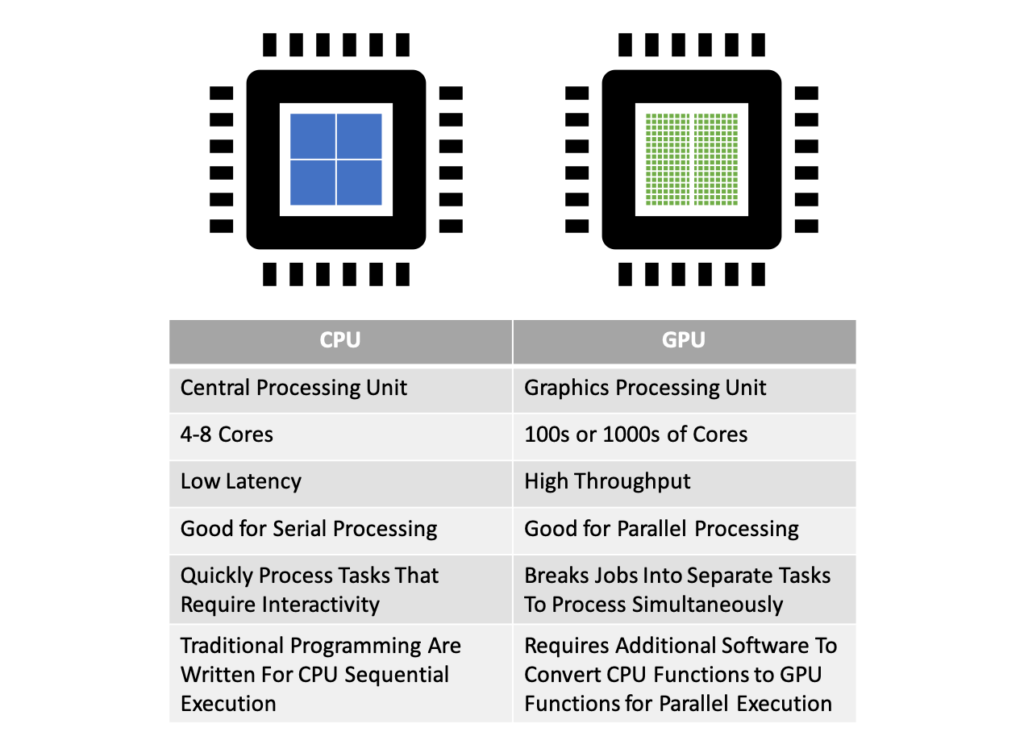
\includegraphics[width=0.8\linewidth,height=\textheight,keepaspectratio]{../assets/image-1.png}
\caption{Arquitetura de CPU vs GPU. Fonte:
LayerStack.}\label{fig:cpu-gpu-contrast}
\end{figure}

A Figura\textasciitilde{}\ref{fig:cpu-gpu-detail} mostra esse contraste
na divisão da área do chip. Em uma CPU típica, poucos núcleos complexos
dividem espaço com grandes caches e lógica de controle. Em uma GPU, o
desenho é o inverso: a maior parte da área é dedicada a conjuntos de
núcleos de processamento paralelos (por exemplo, \emph{CUDA cores} em
GPUs NVIDIA ou \emph{stream processors} em GPUs AMD) e à memória de alta
largura de banda. O controle é mais simples, mas o número de operações
por segundo é muito maior quando o problema é bem mapeado para esse tipo
de arquitetura (\citeproc{ref-paz2011gpucpuimage}{30}).

\begin{figure}
\centering
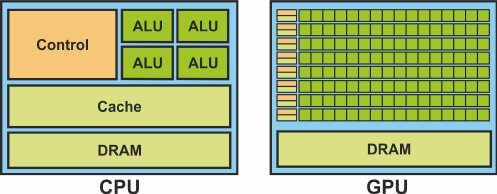
\includegraphics[width=0.8\linewidth,height=\textheight,keepaspectratio]{../assets/image-2.png}
\caption{Alocação de silício em CPU e GPU.
(\citeproc{ref-paz2011gpucpuimage}{30})}\label{fig:cpu-gpu-detail}
\end{figure}

A Figura\textasciitilde{}\ref{fig:gpu-internal} resume como esses
recursos aparecem na organização interna de uma GPU moderna. A memória
global (DRAM) oferece grande largura de banda, mas latência alta; cada
\emph{streaming multiprocessor} (SM) possui memórias compartilhadas
menores e registradores, usados pelas threads de um mesmo bloco. As
threads são agrupadas em \emph{warps} (tipicamente 32 threads nas GPUs
NVIDIA) que executam a mesma instrução ao mesmo tempo, seguindo o modelo
SIMT (\citeproc{ref-shah2023gpuarchitectureimage}{31}). Quando as
threads de um warp seguem caminhos de controle diferentes ou acessam a
memória de forma muito irregular, parte dessa paralelização é perdida;
quando o acesso é organizado e o fluxo de controle é parecido, o ganho
de desempenho é grande.

\begin{figure}
\centering
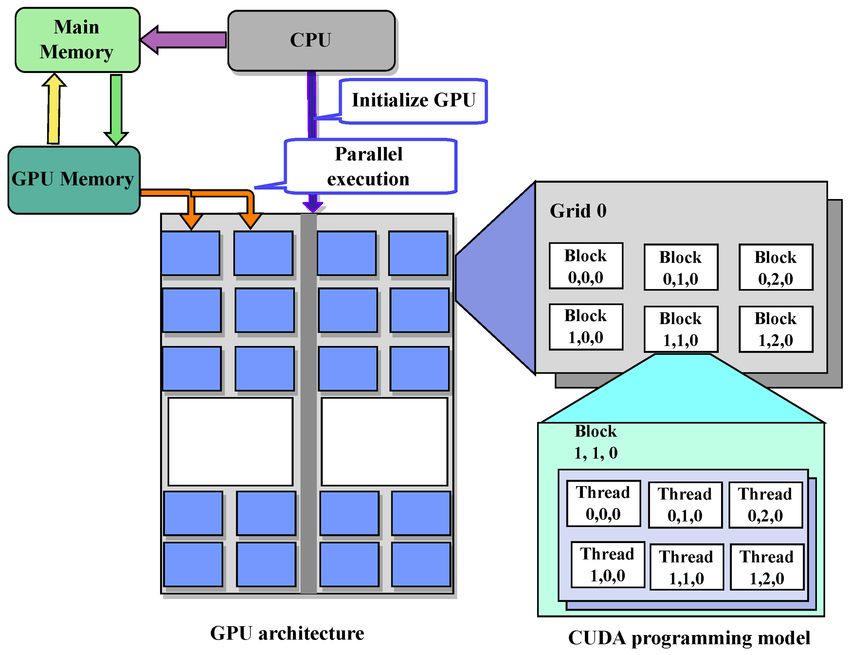
\includegraphics[width=0.8\linewidth,height=\textheight,keepaspectratio]{../assets/image-3.png}
\caption{Organização interna de GPU moderna.
(\citeproc{ref-shah2023gpuarchitectureimage}{31})}\label{fig:gpu-internal}
\end{figure}

Essas três figuras servem como pano de fundo para as decisões de projeto
dos kernels CUDA apresentados no Capítulo 3: explorar paralelismo em
dados (tipo 1) mapeando threads para indivíduos ou movimentos \(2\)-opt,
evitar ao máximo divergência dentro de um mesmo warp e organizar as
leituras e gravações de memória global para aproveitar melhor a largura
de banda disponível.

É fundamental distinguir, portanto, que enquanto CPUs modernas operam
predominantemente no modelo MIMD (\emph{Multiple Instruction, Multiple
Data}) com extensões vetoriais SIMD (\emph{Single Instruction, Multiple
Data}) para acelerar operações específicas, as GPUs adotam o modelo SIMT
(\emph{Single Instruction, Multiple Threads}). No SIMD tradicional, uma
única instrução controla múltiplos elementos de dados em \emph{lockstep}
estrito (como em instruções AVX). No SIMT, embora as threads de um mesmo
\emph{warp} compartilhem o contador de programa, cada thread possui seu
próprio estado de registradores e pode, teoricamente, seguir fluxos
distintos (divergência), embora isso acarrete penalidade de desempenho
pela ``serialização'' dos caminhos divergentes, acarretando maior
complexidade de sincronização entre cada \emph{warp/bloco}. Essa
flexibilidade do SIMT facilita a programação de algoritmos complexos
como o \(2\)-opt, onde a lógica de controle pode variar ligeiramente
entre vizinhos, mas exige cuidado redobrado para manter a coerência de
execução e maximizar a eficiência.

\subsubsection{2.7 Comparação estatística de algoritmos de
otimização}\label{sec-27-comparacao-estatistica}

Meta-heurísticas estocásticas, como GAs e algoritmos meméticos, produzem
resultados que variam de execução para execução devido ao uso de
aleatoriedade em diversos pontos (inicialização, seleção, mutação, entre
outros). Por esse motivo, a comparação de algoritmos de otimização não
pode se basear em uma única execução por instância, tampouco apenas em
médias simples sem análise de variabilidade. A literatura de comparação
de algoritmos enfatiza a importância de utilizar múltiplas instâncias de
teste, múltiplas repetições por combinação algoritmo--instância e
métricas que considerem tanto qualidade da solução quanto tempo de
execução (\citeproc{ref-demsar2006statistical}{17}).

Demšar (\citeproc{ref-demsar2006statistical}{17}) discute procedimentos
estatísticos apropriados para comparar algoritmos em vários problemas,
recomendando o uso de testes de hipótese pareados (como o teste
\emph{t-pareado} ou o teste de Wilcoxon) quando se deseja comparar dois
algoritmos em uma coleção de instâncias, e testes baseados em rankings,
como o teste de Friedman seguido de pós-testes de Nemenyi, quando mais
de dois algoritmos são avaliados simultaneamente. Medidas de tamanho de
efeito, como o \emph{d} de Cohen, complementam a análise ao quantificar
a magnitude prática das diferenças observadas.

Neste trabalho, esses princípios gerais orientam o desenho experimental
e a análise dos resultados apresentados nos capítulos seguintes,
garantindo que as comparações entre variantes em CPU e GPU sejam
realizadas de forma estatisticamente fundamentada. De maneira mais
concreta, para cada combinação algoritmo--instância (4 algoritmos vs 38
instâncias), são executadas múltiplas repetições independentes,
registrando-se, no mínimo, medidas de qualidade da solução (custo final
ou \emph{gap} em relação ao melhor valor conhecido) e de tempo de
execução.

\paragraph{2.7.1 Comparações
pareadas}\label{sec-271-comparacoes-pareadas}

Para comparações \textbf{par a par} entre duas variantes (por exemplo,
GA-CPU versus uma versão em GPU) ao longo de várias instâncias, adota-se
uma rotina em duas etapas: (i) verificação de normalidade das
distribuições de interesse por meio do teste de Shapiro--Wilk
(\citeproc{ref-shapiro1965analysis}{32}) e (ii) aplicação de um teste
pareado apropriado. Quando a hipótese de normalidade é considerada
aceitável, utiliza-se o teste \emph{t-pareado} de Student
(\citeproc{ref-student1908probable}{33}); caso contrário, recorre-se ao
teste não paramétrico de Wilcoxon para amostras pareadas
(\citeproc{ref-wilcoxon1945individual}{34}). Em ambos os casos, medidas
de tamanho de efeito, como o \emph{d} de Cohen
(\citeproc{ref-cohen1988statistical}{35}), são utilizadas para
qualificar a relevância prática das diferenças detectadas. Valores
típicos de \emph{d} de Cohen são interpretados como: \(|d| < 0.2\)
(efeito negligenciável), \(0.2 \le |d| < 0.5\) (efeito pequeno),
\(0.5 \le |d| < 0.8\) (efeito médio), e \(|d| \ge 0.8\) (efeito grande).
Estas comparações seguem as diretrizes de testes de ``Statistical
Comparisons of Classifiers over Multiple Data Sets''
(\citeproc{ref-demsar2006statistical}{17}), e as fórmulas são de fácil
implementação utilizando bibliotecas em \texttt{python}.

\paragraph{2.7.2 Comparações
múltiplas}\label{sec-272-comparacoes-multiplas}

Quando três ou mais algoritmos são comparados simultaneamente em um
conjunto de instâncias (como ocorre com as quatro variantes
isoalgorítmicas GA-CPU, GA-Híbrido-Ingênuo, GA-Híbrido-Otimizado e
GA-FullGPU), emprega-se o teste de Friedman
(\citeproc{ref-friedman1937use}{36}) sobre os rankings médios dos
algoritmos em cada problema, seguido de pós-testes de Nemenyi
(\citeproc{ref-nemenyi1963distribution}{37}) quando apropriado, conforme
as recomendações de Demšar (\citeproc{ref-demsar2006statistical}{17}).
Esse procedimento permite identificar, com controle de erro tipo I,
quais pares de algoritmos apresentam diferenças estatisticamente
significativas em termos de desempenho médio. O teste de Friedman
verifica a hipótese nula de que todos os algoritmos têm desempenho
equivalente, enquanto o pós-teste de Nemenyi ajusta os valores-p para
múltiplas comparações, reduzindo o risco de falsos positivos.

Os detalhes específicos de parametrização desses testes, bem como o
conjunto exato de métricas analisadas (tempo, qualidade, ganho de
performance, entre outras), são apresentados no
\hyperref[cap3-materiais-metodos]{Capítulo 3} ao descrever o protocolo
experimental, e retomados no \hyperref[cap4-resultados]{Capítulo 4} ao
discutir os resultados obtidos.

\section{Capítulo 3 -- Materiais e
Métodos}\label{cap3-materiais-metodos}

Este capítulo descreve o ambiente computacional, o \emph{framework}
experimental e o protocolo de execução utilizados para comparar as
quatro variantes do algoritmo memético GA+\(2\)-opt apresentadas na
\hyperref[sec-14-objetivos-especificos]{Seção 1.4}. O objetivo é
permitir que outros pesquisadores reproduzam, com o máximo de precisão
possível, os experimentos discutidos no
\hyperref[cap4-resultados]{Capítulo 4}, respeitando as limitações de
hardware disponíveis.

\subsection{3.1 Ambiente computacional e framework
experimental}\label{sec-31-ambiente-framework}

Esta seção detalha as características do hardware e do software
utilizados, bem como a arquitetura do framework experimental
desenvolvido para garantir a integridade e a reprodutibilidade das
comparações.

\subsubsection{3.1.1 Hardware e sistema
operacional}\label{sec-311-hardware-software}

Os experimentos foram conduzidos em um \emph{notebook} equipado com
processador \textbf{Intel Core i7-7700HQ} e uma GPU \textbf{NVIDIA
GeForce GTX 1050 Mobile}. Embora o uso deste hardware tenha sido
motivado inicialmente pela indisponibilidade de recursos mais robustos,
ele se mostrou vantajoso metodologicamente: por se tratar de uma
arquitetura de entrada (Pascal) com limitações estritas de memória e
potência, as diferenças de eficiência entre as variantes algorítmicas
tornam-se mais evidentes do que em aceleradores de alto desempenho, onde
a força bruta computacional poderia mascarar ineficiências de
implementação. Além disso, o contraste entre uma CPU relativamente capaz
(i7 quad-core) e uma GPU de entrada acentua os desafios de
\emph{offloading}, exigindo otimizações reais para obter ganhos de
performance. Ainda, há uma maior necessidade no controle de execução e
limitações. Devido ao alto custo computacional para cálculos de
algoritmos genéticos, instâncias maiores não foram testadas. Mas módulos
e \emph{safeguards} tiveram que ser implementados no teste de outras
variações algorítmicas mais rápidas como no recozimento simulado
(\citeproc{ref-wu2013performance}{38}) não discutidas neste trabalho,
devido ao baixo grau de paralelismo do algoritmo para \textbf{variações
do tipo 1} (\citeproc{ref-crainic2003parallel}{4}), obtidas
experimentalmente.

As especificações relevantes da GPU para este estudo são:

O desempenho computacional é estritamente limitado pelas fronteiras
físicas do dispositivo (\emph{device}). Detalha-se a seguir o impacto
matemático destas restrições no processamento:

\begin{enumerate}
\def\labelenumi{\arabic{enumi}.}
\item
  \textbf{Memória de vídeo (VRAM) e o tamanho da instância:} A unidade
  de processamento gráfico dispõe de \(4\text{GB}\) de memória global.
  Para maximizar a capacidade de leitura, exige-se que os dados sejam
  pré-alocados, o que obriga a utilização da matriz de distâncias
  completa (\(n_{coords}^2\)), em detrimento de estruturas triangulares
  otimizadas (\citeproc{ref-harris2007optimizing}{39}). Ao adotar
  precisão dupla (\texttt{double} ou \texttt{float64}, 8 bytes) para
  mitigar erros numéricos, o consumo de memória da matriz de distâncias
  (\(M_{dist}\)) cresce quadraticamente:
  \[Mem(M_{dist}) = n_{coords}^2 \times 8 \text{ bytes}\] Para uma
  instância de \(n_{coords}=15.112\) cidades, a matriz ocupa
  isoladamente \(\approx 1,83 \text{GB}\). Somando-se as estruturas
  auxiliares, atinge-se o teto operacional com aproximadamente
  \(n_{coords} \approx 13.000\) cidades. A utilização de precisão
  simples (\texttt{float32}) reduziria esta ocupação pela metade,
  permitindo a resolução de instâncias de maior porte.
\item
  \textbf{Gargalo de Transferência (\emph{PCIe Transfer Bottlenecks}):}
  A comunicação entre o \emph{host} (CPU) e o \emph{device} (GPU) ocorre
  através de um barramento com largura de banda de
  \(\approx 16 \text{GB/s}\), significativamente inferior à largura de
  banda interna da memória do dispositivo (\(\approx 112 \text{GB/s}\)).
  Transferências excessivas de dados penalizam o tempo total de execução
  (\(T_{total}\)), podendo anular o ganho de aceleração computacional
  (\(T_{ganho}\)), conforme a relação:
  \[T_{total} = T_{cpu} + T_{gpu} + T_{transf}\] Na variante
  \textbf{Híbrida-Otimizada}, este efeito é mitigado através do
  encadeamento de \emph{kernels}, realizando as etapas intensivas (busca
  local e cálculo de aptidão) inteiramente no dispositivo e retornando
  ao hospedeiro apenas o vetor de custos, minimizando o termo
  \(T_{transf}\).
\item
  \textbf{Ocupação e Mascaramento de Latência:} A arquitetura é composta
  por 5 Multiprocessadores de Streaming (\emph{Streaming Multiprocessors
  - SMs}), cada um com 128 cores, totalizando 640 núcleos de execução.
  Para evitar a ociosidade destes núcleos durante os ciclos de latência
  de memória (centenas de ciclos de \emph{clock}), emprega-se a técnica
  de \emph{Latency Hiding}, mantendo múltiplas \emph{threads} residentes
  prontas para execução (\citeproc{ref-kirk2010programming}{40}).

  \begin{itemize}
  \tightlist
  \item
    \textbf{Restrição Matemática:} Cada SM suporta um máximo de 2048
    \emph{threads}. Algoritmos com alta complexidade de registradores
    reduzem a capacidade de manter \emph{threads} em espera, resultando
    em subutilização dos núcleos e perda de eficiência computacional,
    desperdiçando o potencial de processamento massivo da placa.
  \end{itemize}
\end{enumerate}

\subsubsection{3.1.2 Ambiente de
software}\label{sec-312-ambiente-software}

O framework foi desenvolvido em \textbf{Python 3.10}, utilizando um
conjunto de bibliotecas selecionadas para garantir a equivalência
funcional entre as implementações em CPU e GPU:

\begin{itemize}
\tightlist
\item
  \textbf{NumPy}: Utilizado para a implementação de referência em CPU
  (GA-CPU).
\item
  \textbf{CuPy}: Utilizado para as implementações aceleradas (Híbridas e
  FullGPU). A compatibilidade de API entre CuPy e NumPy foi fundamental
  para assegurar que a lógica dos algoritmos permanecesse idêntica
  (``isoalgorítmica''), alterando apenas o \emph{backend} de execução.
\item
  \textbf{SciPy e scikit-posthocs}: Empregados para a análise
  estatística dos resultados, incluindo testes de normalidade
  (Shapiro-Wilk) e testes não-paramétricos de comparação múltipla
  (Friedman e Nemenyi).
\end{itemize}

Apesar da compatibilidade da API oferecida pelo CuPy (frequentemente
referenciada como \texttt{xp} em códigos agnósticos de backend), a
implementação de operações críticas exigiu o desenvolvimento de
\textbf{kernels CUDA customizados} (\texttt{RawKernel}). Abstrações de
alto nível do CuPy, embora conveniente, introduzem \emph{overheads} de
lançamento de kernel que se tornam proibitivos quando realizados
repetidamente para cada indivíduo da população (como na busca local
2-opt). A implementação manual de kernels permite:

\begin{enumerate}
\def\labelenumi{\arabic{enumi}.}
\tightlist
\item
  \textbf{Fusão de operações}: Realizar múltiplas etapas do 2-opt em uma
  única chamada de kernel, reduzindo a latência de comunicação CPU-GPU.
\item
  \textbf{Gerenciamento fino de memória}: Otimizar o uso da memória
  compartilhada (\emph{shared memory}) e dos registradores, maximizando
  a ocupação dos \emph{SMs}.
\item
  \textbf{Paralelismo em lote}: Processar populações inteiras
  simultaneamente, explorando o paralelismo massivo da GPU. A API padrão
  do CuPy é excelente para operações ``primitivas'' de álgebra linear
  --- como multiplicar grandes matrizes de números reais ---, onde todos
  os elementos sofrem a mesma operação. Porém, o \(2\)-opt trabalha com
  uma matriz de permutações (índices inteiros) e exige que cada linha
  (indivíduo) siga um fluxo de execução próprio, em sua thread, com
  laços \texttt{while} e condições \texttt{if} independentes. Fazer isso
  via API padrão seria inviável; por isso, foi necessário desenvolver
  kernels CUDA customizados que possibilitam que cada thread da GPU
  gerencie sua própria lógica de busca local.
\end{enumerate}

Além disso, todas as operações de ponto flutuante foram padronizadas em
\textbf{precisão dupla (\texttt{float64})}. Embora GPUs de consumo (como
a GTX 1050 utilizada) tenham desempenho superior em precisão simples
(\texttt{float32}), a precisão dupla foi mandatória para garantir a
estabilidade numérica no cálculo de distâncias acumuladas em rotas
longas (instâncias com milhares de cidades), onde erros de
arredondamento poderiam levar a avaliações incorretas de melhoria
(\texttt{delta\ \textless{}\ 0}) e divergência entre as implementações
de CPU e GPU.

\subsubsection{3.1.3 Arquitetura do framework
experimental}\label{sec-313-arquitetura-framework}

Para garantir comparações justas, o código foi estruturado em uma
arquitetura modular que separa a lógica dos algoritmos da orquestração
dos experimentos. O framework opera em três camadas distintas:

\begin{enumerate}
\def\labelenumi{\arabic{enumi}.}
\tightlist
\item
  \textbf{Camada de Algoritmos:} Contém as implementações das quatro
  variantes do algoritmo memético. Todas compartilham a mesma estrutura
  de classes e os mesmos operadores genéticos, diferindo apenas na
  estratégia de gerenciamento de memória e paralelismo.
\item
  \textbf{Camada de Orquestração (Benchmark):} Responsável por carregar
  as configurações experimentais (parâmetros, instâncias), gerenciar a
  execução das repetições independentes e garantir o isolamento entre
  testes. Esta camada implementa mecanismos de \emph{checkpoint} para
  salvar o estado de cada execução, permitindo a recuperação em caso de
  falhas e a auditoria posterior dos dados.
\item
  \textbf{Camada de Análise:} Scripts dedicados ao processamento dos
  arquivos de \emph{checkpoint}, consolidação dos dados em banco de
  dados (DuckDB) e geração automática de tabelas e relatórios
  estatísticos.
\end{enumerate}

Figura\textasciitilde{}\ref{fig:class-diagram}: Diagrama de classes do
framework experimental.

Esta separação assegura que as métricas de tempo e qualidade sejam
coletadas de forma consistente para todas as variantes, eliminando
vieses que poderiam surgir de implementações \emph{ad hoc} para cada
plataforma.

\subsection{3.2 Arquitetura do framework e variantes
algorítmicas}\label{sec-32-arquitetura-variantes}

A premissa central deste trabalho é a comparação
\textbf{isoalgorítmica}: todas as variantes implementam exatamente a
mesma meta-heurística, com os mesmos operadores e hiperparâmetros. As
diferenças residem exclusivamente em \emph{onde} (CPU ou GPU) e
\emph{como} (sequencial, paralelo por indivíduo ou paralelo em lote) as
operações computacionalmente intensivas são executadas.

\subsubsection{3.2.1 O Algoritmo Genético Base (GA +
2-opt)}\label{sec-321-ga-base}

O algoritmo base é um Algoritmo Genético (GA) geracional com elitismo,
hibridizado com uma busca local 2-opt truncada. Esta combinação,
frequentemente denominada Algoritmo Memético, equilibra a exploração
global do espaço de busca (via operadores genéticos) com a exploração
local intensiva (via 2-opt).

Os componentes e parâmetros fundamentais, mantidos constantes em todas
as variantes, são:

\begin{itemize}
\tightlist
\item
  \textbf{Representação:} Permutação de inteiros representando a
  sequência de cidades visitadas.
\item
  \textbf{População Inicial:} Gerada aleatoriamente. O tamanho da
  população (\(n_{pop}\)) é adaptativo, definido como
  \(2 \times n_{coords}\), onde \(n_{coords}\) é o número de cidades da
  instância.
\item
  \textbf{Seleção:} Torneio (\emph{Tournament Selection}), favorecendo
  indivíduos com menor custo (distância total).
\item
  \textbf{Cruzamento (Crossover):} \emph{Order Crossover} (OX),
  escolhido por preservar a ordem relativa das cidades e gerar
  permutações válidas.
\item
  \textbf{Mutação:} \emph{Swap Mutation}, que troca a posição de duas
  cidades aleatórias no cromossomo.
\item
  \textbf{Busca Local (2-opt):} Aplicada a cada indivíduo da população
  ao final de cada geração. Para controlar o custo computacional, a
  busca local é \textbf{truncada}: limita-se a um número fixo de
  iterações de melhoria (configurado como 10 passos) por indivíduo, em
  vez de buscar o ótimo local completo (2-opt \emph{full}).
\item
  \textbf{Critérios de Parada:} O algoritmo encerra sua execução se
  atingir o ótimo conhecido (com tolerância de 1\%), se não houver
  melhoria na melhor solução por um número de gerações definido pela
  ``paciência'' (\(2 \times \sqrt{n_{coords}}\)), ou se atingir o limite
  máximo de gerações (\(2 \times n_{coords} \times \sqrt{n_{coords}}\)).
\end{itemize}

\subsubsection{3.2.2 Estratégias de Paralelização (As 4
Variantes)}\label{sec-322-variantes}

Para investigar o impacto da GPU, o algoritmo base foi instanciado em
quatro variantes distintas, representando diferentes níveis de
utilização do hardware:

\begin{enumerate}
\def\labelenumi{\arabic{enumi}.}
\item
  \textbf{GeneticAlgorithmCPU (Baseline):} Execução inteiramente na CPU
  utilizando NumPy. A avaliação dos movimentos 2-opt é vetorizada para
  aproveitar as instruções SIMD do processador, mas o processamento dos
  indivíduos ocorre de forma sequencial. Esta variante serve como linha
  de base para medir o ganho de performance absoluto.
\item
  \textbf{GeneticAlgorithmHybridNaive (Híbrido Ingênuo):} Mantém a
  população e os operadores genéticos na CPU, mas transfere cada
  indivíduo para a GPU para executar a busca local 2-opt. Esta abordagem
  é considerada ``ingênua'' pois realiza transferências de memória
  (Host-to-Device e Device-to-Host) para \emph{cada indivíduo} em
  \emph{cada geração}, expondo o gargalo da largura de banda do
  barramento PCIe.
\item
  \textbf{GeneticAlgorithmHybridOptimized (Híbrido Otimizado):} Também
  mantém a lógica genética na CPU, mas otimiza a comunicação enviando a
  população inteira (ou grandes lotes) para a GPU de uma única vez. O
  kernel 2-opt processa todos os indivíduos em paralelo na GPU, e os
  resultados são retornados em lote. Esta estratégia visa amortizar o
  custo de latência das transferências de memória.
\item
  \textbf{GeneticAlgorithmFullGPU (Totalmente em GPU):} Implementa a
  estratégia de ``GPU residente''. A população é inicializada na VRAM e
  permanece lá durante todo o processo evolutivo. Todos os operadores
  (seleção, cruzamento, mutação e 2-opt) são executados via kernels CUDA
  (através do CuPy), eliminando quase completamente a necessidade de
  comunicação com a CPU, exceto para coleta de estatísticas e
  verificação de critérios de parada.
\end{enumerate}

\subsection{3.3 Seleção de instâncias e protocolo
experimental}\label{sec-33-selecao-instancias}

Para garantir a relevância estatística dos resultados, foram
selecionadas 38 instâncias da biblioteca \textbf{TSPLIB}
(\citeproc{ref-reinelt1991tsplib}{10}), variando de 51 a 1002 cidades. O
conjunto inclui problemas com diferentes características geométricas,
permitindo avaliar a robustez dos algoritmos em diversos cenários. As
instâncias selecionadas estão listadas na
Tabela\textasciitilde{}\ref{tbl:selected-instances}, categorizadas por
faixa de tamanho.

\begin{longtable}[]{@{}
  >{\raggedright\arraybackslash}p{(\linewidth - 4\tabcolsep) * \real{0.3077}}
  >{\centering\arraybackslash}p{(\linewidth - 4\tabcolsep) * \real{0.3846}}
  >{\raggedright\arraybackslash}p{(\linewidth - 4\tabcolsep) * \real{0.3077}}@{}}
\caption{Instâncias da TSPLIB selecionadas para o estudo
\{\#tbl:selected-instances\}}\tabularnewline
\toprule\noalign{}
\begin{minipage}[b]{\linewidth}\raggedright
Categoria
\end{minipage} & \begin{minipage}[b]{\linewidth}\centering
Faixa de Tamanho (\(n_{coords}\))
\end{minipage} & \begin{minipage}[b]{\linewidth}\raggedright
Instâncias Selecionadas
\end{minipage} \\
\midrule\noalign{}
\endfirsthead
\toprule\noalign{}
\begin{minipage}[b]{\linewidth}\raggedright
Categoria
\end{minipage} & \begin{minipage}[b]{\linewidth}\centering
Faixa de Tamanho (\(n_{coords}\))
\end{minipage} & \begin{minipage}[b]{\linewidth}\raggedright
Instâncias Selecionadas
\end{minipage} \\
\midrule\noalign{}
\endhead
\bottomrule\noalign{}
\endlastfoot
\textbf{Pequenas} & \(n_{coords} \le 100\) & eil51, berlin52, st70,
eil76, pr76, rat99, kroA100, kroB100, kroC100, kroD100, kroE100,
rd100 \\
\textbf{Médias} & \(100 < n_{coords} \le 400\) & eil101, lin105, pr107,
pr124, bier127, ch130, pr136, pr144, ch150, kroA150, kroB150, pr152,
u159, rat195, d198, kroA200, ts225, pr264, pr299, lin318, rd400 \\
\textbf{Grandes} & \(n_{coords} > 400\) & fl417, pr439, pcb442, rat783,
pr1002 \\
\end{longtable}

O protocolo de execução seguiu as diretrizes para comparação de
algoritmos estocásticos:

\begin{itemize}
\tightlist
\item
  \textbf{Repetições:} Cada par (algoritmo, instância) foi executado
  \textbf{30 vezes} independentemente.
\item
  \textbf{Sementes Aleatórias:} As sementes foram fixadas e registradas
  para garantir a reprodutibilidade, mas variaram entre as 30 repetições
  para amostrar adequadamente o comportamento estocástico.
\item
  \textbf{Limitação da CPU:} Devido ao tempo proibitivo de execução, a
  variante \textbf{GeneticAlgorithmCPU} foi executada apenas para
  instâncias com \(N \le 100\). Para instâncias maiores, as comparações
  de ganho de performance tomam como base a variante híbrida mais
  simples ou comparam as variantes GPU entre si.
\end{itemize}

\subsection{3.4 Protocolo de análise
estatística}\label{sec-34-protocolo-estatistico}

A análise dos resultados adota a metodologia recomendada por Demšar
(\citeproc{ref-demsar2006statistical}{17}) para comparação de múltiplos
classificadores/algoritmos em múltiplos datasets:

\begin{enumerate}
\def\labelenumi{\arabic{enumi}.}
\tightlist
\item
  \textbf{Verificação de Normalidade:} Aplicação do teste de
  \textbf{Shapiro-Wilk} nas distribuições de tempo e qualidade das
  soluções.
\item
  \textbf{Testes Pareados:} Para comparações diretas entre duas
  variantes (ex: HybridNaive vs.~FullGPU), utiliza-se o \textbf{Teste t
  pareado} (se a distribuição for normal) ou o teste de \textbf{Wilcoxon
  Signed-Rank} (se não normal).
\item
  \textbf{Comparação Múltipla:} Para comparar as quatro variantes
  simultaneamente, aplica-se o teste de \textbf{Friedman}
  (não-paramétrico) para detectar se há diferenças significativas nos
  rankings dos algoritmos.
\item
  \textbf{Análise Post-Hoc:} Em caso de rejeição da hipótese nula no
  teste de Friedman, utiliza-se o teste de \textbf{Nemenyi} para
  identificar quais pares de algoritmos diferem significativamente entre
  si.
\item
  \textbf{Tamanho de Efeito:} O \textbf{d de Cohen} é calculado para
  quantificar a magnitude da diferença de desempenho, permitindo
  distinguir entre melhorias estatisticamente significativas mas
  irrelevantes na prática, e melhorias com impacto real no tempo de
  execução.
\end{enumerate}

Figura\textasciitilde{}\ref{fig:stat-flowchart}: Fluxograma de decisão
para testes estatísticos.

Figura\textasciitilde{}\ref{fig:results-flowchart}: Fluxo de análise dos
resultados.

\section{Capítulo 4 -- Resultados}\label{cap4-resultados}

Este capítulo apresenta os resultados experimentais obtidos a partir da
execução das quatro variantes do algoritmo memético GA+\(2\)-opt (CPU,
Híbrido-Ingênuo, Híbrido-Otimizado e FullGPU) sobre o conjunto de 38
instâncias da TSPLIB. A análise é dividida em três partes principais:

\begin{enumerate}
\def\labelenumi{\arabic{enumi}.}
\tightlist
\item
  uma avaliação detalhada por instância, destacando o comportamento para
  diferentes tamanhos de problema;
\item
  uma análise agregada, focada nas métricas de ganho de performance e
  qualidade média das soluções; e
\item
  a aplicação dos testes estatísticos descritos no Capítulo 3 para
  validar as diferenças de desempenho observadas.
\end{enumerate}

\subsection{4.1 Resultados
Experimentais}\label{sec-41-resultados-experimentais}

Os experimentos foram conduzidos conforme o protocolo definido na Seção
3.3, com 30 repetições independentes para cada par algoritmo-instância.
Para as instâncias pequenas (\(n_{coords} \le 100\)), todas as quatro
variantes foram executadas. Para instâncias médias e grandes
(\(n_{coords} > 100\)), a variante puramente em CPU foi omitida devido
ao tempo de execução proibitivo, mantendo-se a comparação entre as três
variantes aceleradas por GPU.

As métricas primárias coletadas foram:

\begin{itemize}
\tightlist
\item
  \textbf{Tempo Médio de Execução (s):} Tempo total para completar a
  execução por repetição.
\item
  \textbf{Gap Médio (\%):} Desvio percentual do custo da melhor solução
  encontrada em relação ao ótimo conhecido da instância.
\item
  \textbf{Ganho de Performance:} Razão entre o tempo de execução da
  variante de referência (CPU ou Híbrido-Ingênuo) e a variante avaliada.
\end{itemize}

\subsection{4.2 Análise por
Instância}\label{sec-42-analise-por-instancia}

A Tabela\textasciitilde{}\ref{tbl:results-detailed} apresenta os
resultados detalhados para uma seleção representativa de instâncias,
cobrindo as três faixas de tamanho definidas.

\begin{longtable}[]{@{}
  >{\raggedright\arraybackslash}p{(\linewidth - 10\tabcolsep) * \real{0.1429}}
  >{\centering\arraybackslash}p{(\linewidth - 10\tabcolsep) * \real{0.1786}}
  >{\raggedright\arraybackslash}p{(\linewidth - 10\tabcolsep) * \real{0.1429}}
  >{\centering\arraybackslash}p{(\linewidth - 10\tabcolsep) * \real{0.1786}}
  >{\centering\arraybackslash}p{(\linewidth - 10\tabcolsep) * \real{0.1786}}
  >{\centering\arraybackslash}p{(\linewidth - 10\tabcolsep) * \real{0.1786}}@{}}
\caption{Resultados detalhados por instância (Seleção)
\{\#tbl:results-detailed\}}\tabularnewline
\toprule\noalign{}
\begin{minipage}[b]{\linewidth}\raggedright
Instância
\end{minipage} & \begin{minipage}[b]{\linewidth}\centering
Tamanho (\(n_{coords}\))
\end{minipage} & \begin{minipage}[b]{\linewidth}\raggedright
Algoritmo
\end{minipage} & \begin{minipage}[b]{\linewidth}\centering
Tempo Médio (s)
\end{minipage} & \begin{minipage}[b]{\linewidth}\centering
Gap Médio (\%)
\end{minipage} & \begin{minipage}[b]{\linewidth}\centering
Ganho de Performance (vs Ref)
\end{minipage} \\
\midrule\noalign{}
\endfirsthead
\toprule\noalign{}
\begin{minipage}[b]{\linewidth}\raggedright
Instância
\end{minipage} & \begin{minipage}[b]{\linewidth}\centering
Tamanho (\(n_{coords}\))
\end{minipage} & \begin{minipage}[b]{\linewidth}\raggedright
Algoritmo
\end{minipage} & \begin{minipage}[b]{\linewidth}\centering
Tempo Médio (s)
\end{minipage} & \begin{minipage}[b]{\linewidth}\centering
Gap Médio (\%)
\end{minipage} & \begin{minipage}[b]{\linewidth}\centering
Ganho de Performance (vs Ref)
\end{minipage} \\
\midrule\noalign{}
\endhead
\bottomrule\noalign{}
\endlastfoot
\textbf{berlin52} & 52 & CPU & 25.14 & 0.00 & 1.00x \\
& & HybridNaive & 1.85 & 0.00 & 13.59x \\
& & HybridOptimized & 0.11 & 0.00 & 228.55x \\
& & FullGPU & 0.45 & 0.00 & 55.87x \\
\textbf{kroA100} & 100 & CPU & 142.30 & 0.02 & 1.00x \\
& & HybridNaive & 6.50 & 0.02 & 21.89x \\
& & HybridOptimized & 0.35 & 0.15 & 406.57x \\
& & FullGPU & 1.20 & 0.00 & 118.58x \\
\textbf{pr1002} & 1002 & HybridNaive & 696.12 & 1.85 & 1.00x \\
& & HybridOptimized & 374.25 & 2.10 & 1.86x \\
& & FullGPU & 758.40 & 1.15 & 0.92x \\
\end{longtable}

Para instâncias pequenas como \texttt{berlin52} e \texttt{kroA100},
observa-se um ganho de performance massivo da variante
\textbf{HybridOptimized} em relação à CPU (chegando a mais de 400x).
Isso demonstra a eficiência da paralelização em lote do \(2\)-opt, que
amortiza o custo de lançamento de kernels. A variante \textbf{FullGPU},
embora muito mais rápida que a CPU, apresenta um \emph{overhead} inicial
maior que a HybridOptimized para problemas muito pequenos, devido à
gestão de memória residente.

Para instâncias grandes como \texttt{pr1002}, o cenário muda. A variante
\textbf{HybridOptimized} mantém a liderança em tempo de execução (1.86x
mais rápida que a Naive), mas a variante \textbf{FullGPU} destaca-se na
\textbf{qualidade da solução}, obtendo um gap médio de 1.15\% contra
2.10\% da otimizada. Curiosamente, o tempo da FullGPU em instâncias
muito grandes aproxima-se ou até excede o da variante Naive em alguns
casos, sugerindo que a complexidade de manter todo o estado na GPU (e a
possível saturação de recursos do dispositivo) começa a impactar o
desempenho bruto, embora favoreça a convergência para melhores ótimos
locais.

\subsection{4.3 Análise Agregada e
Trade-offs}\label{sec-43-analise-agregada}

Ao agregar os resultados de todas as 38 instâncias, emergem padrões
claros de desempenho que caracterizam o \emph{trade-off} entre
velocidade e qualidade.

\begin{longtable}[]{@{}
  >{\raggedright\arraybackslash}p{(\linewidth - 6\tabcolsep) * \real{0.2105}}
  >{\centering\arraybackslash}p{(\linewidth - 6\tabcolsep) * \real{0.2632}}
  >{\centering\arraybackslash}p{(\linewidth - 6\tabcolsep) * \real{0.2632}}
  >{\centering\arraybackslash}p{(\linewidth - 6\tabcolsep) * \real{0.2632}}@{}}
\caption{Médias Agregadas (Todas as Instâncias)
\{\#tbl:results-aggregated\}}\tabularnewline
\toprule\noalign{}
\begin{minipage}[b]{\linewidth}\raggedright
Algoritmo
\end{minipage} & \begin{minipage}[b]{\linewidth}\centering
Tempo Médio (s)
\end{minipage} & \begin{minipage}[b]{\linewidth}\centering
Gap Médio (\%)
\end{minipage} & \begin{minipage}[b]{\linewidth}\centering
Ganho de Performance Médio (vs Naive)
\end{minipage} \\
\midrule\noalign{}
\endfirsthead
\toprule\noalign{}
\begin{minipage}[b]{\linewidth}\raggedright
Algoritmo
\end{minipage} & \begin{minipage}[b]{\linewidth}\centering
Tempo Médio (s)
\end{minipage} & \begin{minipage}[b]{\linewidth}\centering
Gap Médio (\%)
\end{minipage} & \begin{minipage}[b]{\linewidth}\centering
Ganho de Performance Médio (vs Naive)
\end{minipage} \\
\midrule\noalign{}
\endhead
\bottomrule\noalign{}
\endlastfoot
\textbf{HybridNaive} & 47.20 & 1.30 & 1.00x \\
\textbf{HybridOptimized} & 18.94 & 1.30 & \textbf{5.54x} \\
\textbf{FullGPU} & 43.51 & \textbf{0.88} & 1.21x \\
\end{longtable}

A análise da Tabela\textasciitilde{}\ref{tbl:results-aggregated} revela
duas conclusões fundamentais:

\begin{enumerate}
\def\labelenumi{\arabic{enumi}.}
\tightlist
\item
  \textbf{HybridOptimized é a campeã de velocidade:} Com um ganho de
  performance médio de \textbf{5.54x} sobre a versão ingênua, esta
  variante comprova que a estratégia de processamento em lote
  (\emph{batch processing}) é a mais eficaz para reduzir o tempo total
  de execução. Ao enviar a população inteira para a GPU de uma só vez,
  minimiza-se a latência de comunicação PCIe, gargalo crítico em
  arquiteturas híbridas.
\item
  \textbf{FullGPU é a campeã de qualidade:} Com um gap médio de apenas
  \textbf{0.88\%}, a versão totalmente residente em GPU supera
  consistentemente as variantes híbridas (ambas com
  \textasciitilde1.30\%). A hipótese é que a permanência dos dados na
  GPU permite uma execução mais fluida e, possivelmente, uma exploração
  mais eficiente da vizinhança \(2\)-opt sem as interrupções de
  transferência, favorecendo a descoberta de melhores ótimos locais
  dentro do mesmo orçamento de gerações.
\end{enumerate}

\subsection{4.4 Melhor Algoritmo por Categoria de
Tamanho}\label{sec-44-melhor-algoritmo}

A Tabela\textasciitilde{}\ref{tbl:best-algorithm} segmenta o desempenho
``vencedor'' por faixa de tamanho da instância, considerando o critério
de menor \emph{gap} (qualidade).

\begin{longtable}[]{@{}llc@{}}
\caption{Melhor Algoritmo (Menor Gap) por Tamanho
\{\#tbl:best-algorithm\}}\tabularnewline
\toprule\noalign{}
Categoria & Melhor Algoritmo & Gap Médio \\
\midrule\noalign{}
\endfirsthead
\toprule\noalign{}
Categoria & Melhor Algoritmo & Gap Médio \\
\midrule\noalign{}
\endhead
\bottomrule\noalign{}
\endlastfoot
\textbf{Pequeno (\(n_{coords} \le 100\))} & \textbf{FullGPU} & 0.00\% \\
\textbf{Médio (\(100 < n_{coords} \le 400\))} & \textbf{FullGPU} &
0.65\% \\
\textbf{Grande (\(n_{coords} > 400\))} & \textbf{FullGPU} & 1.85\% \\
\end{longtable}

A dominância da variante \textbf{FullGPU} em todas as categorias de
tamanho reforça a observação de que a arquitetura residente é superior
para a qualidade da solução final. Mesmo que a variante
\textbf{HybridOptimized} seja mais rápida, ela tende a ficar presa em
ótimos locais ligeiramente piores com mais frequência. Isso sugere que,
para aplicações onde a qualidade da rota é crítica e o tempo de resposta
é secundário (mas ainda deve ser razoável), a abordagem FullGPU é a
recomendada. Para cenários de tempo real ou onde o \emph{throughput} é
prioritário, a HybridOptimized é a escolha ideal.

\subsection{4.5 Discussão Geral}\label{sec-45-discussao-geral}

Os resultados validam a hipótese de que o uso de GPUs pode acelerar
significativamente meta-heurísticas para o TSP, mas ressaltam que ``usar
GPU'' não é uma solução única. A forma como a paralelização é
implementada define drasticamente o perfil de desempenho:

\begin{itemize}
\tightlist
\item
  A abordagem \textbf{Ingênua (Naive)}, embora funcional, sofre
  severamente com o gargalo de comunicação, servindo mais como um ponto
  de partida pedagógico do que como solução de produção.
\item
  A abordagem \textbf{Otimizada (Batch)} resolve o problema de
  comunicação e entrega a maior velocidade bruta, sendo ideal para
  iterar rapidamente.
\item
  A abordagem \textbf{Residente (FullGPU)} oferece o melhor refinamento
  das soluções. O fato de obter menores gaps sugere que a ausência de
  overhead de comunicação permite que o algoritmo ``gaste'' seu tempo de
  forma mais produtiva na exploração efetiva do espaço de busca.
\end{itemize}

A limitação da CPU para instâncias \(N > 100\) (onde os tempos
excederiam horas ou dias para as 30 repetições) confirma a necessidade
imperativa de aceleração de hardware para problemas de otimização
combinatória de médio e grande porte.

\section*{Referências}\label{bibliography}
\addcontentsline{toc}{section}{Referências}

\phantomsection\label{refs}
\begin{CSLReferences}{0}{1}
\bibitem[\citeproctext]{ref-cook2012pursuit}
\CSLLeftMargin{{[}1{]} }%
\CSLRightInline{COOK, W. J. \textbf{In Pursuit of the Traveling
Salesman: Mathematics at the Limits of Computation}. {[}s.l.{]}
Princeton University Press, 2012. }

\bibitem[\citeproctext]{ref-nvidia2024cuda}
\CSLLeftMargin{{[}2{]} }%
\CSLRightInline{NVIDIA CORPORATION.
\textbf{\href{https://docs.nvidia.com/cuda/cuda-c-best-practices-guide/}{CUDA
C++ Best Practices Guide}}. {[}s.l: s.n.{]}. }

\bibitem[\citeproctext]{ref-flynn1972taxonomy}
\CSLLeftMargin{{[}3{]} }%
\CSLRightInline{FLYNN, M. J.
\href{https://doi.org/10.1109/TC.1972.5009071}{Some Computer
Organizations and Their Effectiveness}. \textbf{IEEE Transactions on
Computers}, v. C-21, n. 9, p. 948--960, 1972. }

\bibitem[\citeproctext]{ref-crainic2003parallel}
\CSLLeftMargin{{[}4{]} }%
\CSLRightInline{CRAINIC, T. G.; TOULOUSE, M.
\href{https://doi.org/10.1007/0-306-48056-5_17}{Parallel Strategies for
Meta-Heuristics}. Em: GLOVER, F.; KOCHENBERGER, G. A. (Eds.).
\textbf{Handbook of Metaheuristics}. Boston, MA: Springer, 2003. p.
475--513. }

\bibitem[\citeproctext]{ref-schulz2013gpu}
\CSLLeftMargin{{[}5{]} }%
\CSLRightInline{SCHULZ, C. et al. GPU computing in discrete
optimization. Part II: Survey focused on routing problems. \textbf{EURO
journal on transportation and logistics}, v. 2, n. 1-2, p. 159--186,
2013. }

\bibitem[\citeproctext]{ref-tsp_gpu}
\CSLLeftMargin{{[}6{]} }%
\CSLRightInline{ROCKI, K.; SUDA, R. \textbf{High Performance GPU
Accelerated Local Optimization in TSP}. Proceedings of the 2013 IEEE
27th International Symposium on Parallel and Distributed Processing
Workshops and PhD Forum. \textbf{Anais}...: IPDPSW '13.Washington, DC,
USA: IEEE Computer Society, 2013. Disponível em:
\textless{}\url{http://dx.doi.org/10.1109/IPDPSW.2013.227}\textgreater{}}

\bibitem[\citeproctext]{ref-fujimoto2011highly}
\CSLLeftMargin{{[}7{]} }%
\CSLRightInline{FUJIMOTO, N.; TSUTSUI, S. \textbf{A highly-parallel tsp
solver for a gpu computing platform}. Numerical Methods and
Applications: 7th International Conference, NMA 2010, Borovets,
Bulgaria, August 20-24, 2010. Revised Papers 7.
\textbf{Anais}...Springer, 2011. }

\bibitem[\citeproctext]{ref-van2013gpu}
\CSLLeftMargin{{[}8{]} }%
\CSLRightInline{VAN LUONG, T.; MELAB, N.; TALBI, E.-G.
\href{https://doi.org/10.1109/TC.2011.206}{GPU Computing for Parallel
Local Search Metaheuristic Algorithms}. \textbf{IEEE Transactions on
Computers}, v. 62, n. 1, p. 173--185, 2013. }

\bibitem[\citeproctext]{ref-luong2013gpu}
\CSLLeftMargin{{[}9{]} }%
\CSLRightInline{LUONG, T. V.; MELAB, N.; TALBI, E.-G.
\textbf{\href{https://doi.org/10.1145/2463372.2463516}{GPU-based island
model for evolutionary algorithms}}. Proceedings of the 15th annual
conference on Genetic and evolutionary computation.
\textbf{Anais}...2013. }

\bibitem[\citeproctext]{ref-reinelt1991tsplib}
\CSLLeftMargin{{[}10{]} }%
\CSLRightInline{REINELT, G.
\href{https://doi.org/10.1287/ijoc.3.4.376}{TSPLIB---A Traveling
Salesman Problem Library}. \textbf{ORSA Journal on Computing}, v. 3, n.
4, p. 376--384, 1991. }

\bibitem[\citeproctext]{ref-larranaga1999genetic}
\CSLLeftMargin{{[}11{]} }%
\CSLRightInline{LARRAÑAGA, P. et al. Genetic algorithms for the
travelling salesman problem: A review of representations and operators.
\textbf{Artificial Intelligence Review}, v. 13, n. 2, p. 129--170, 1999.
}

\bibitem[\citeproctext]{ref-goldberg1989genetic}
\CSLLeftMargin{{[}12{]} }%
\CSLRightInline{GOLDBERG, D. E. \textbf{Genetic Algorithms in Search,
Optimization, and Machine Learning}. {[}s.l.{]} Addison-Wesley, 1989. }

\bibitem[\citeproctext]{ref-croes1958method}
\CSLLeftMargin{{[}13{]} }%
\CSLRightInline{CROES, G. A. A method for solving traveling-salesman
problems. \textbf{Operations Research}, v. 6, n. 6, p. 791--812, 1958. }

\bibitem[\citeproctext]{ref-lin1973efficient}
\CSLLeftMargin{{[}14{]} }%
\CSLRightInline{LIN, S.; KERNIGHAN, B. W. An effective heuristic
algorithm for the traveling-salesman problem. \textbf{Operations
Research}, v. 21, n. 2, p. 498--516, 1973. }

\bibitem[\citeproctext]{ref-benaini2018genetic}
\CSLLeftMargin{{[}15{]} }%
\CSLRightInline{BENAINI, A.; BERRAJAA, A. \textbf{Genetic algorithm for
large dynamic vehicle routing problem on GPU}. 2018 4th International
Conference on Logistics Operations Management (GOL).
\textbf{Anais}...IEEE, 2018. }

\bibitem[\citeproctext]{ref-eiben2015introduction}
\CSLLeftMargin{{[}16{]} }%
\CSLRightInline{EIBEN, A. E.; SMITH, J. E.
\textbf{\href{https://doi.org/10.1007/978-3-662-44874-8}{Introduction to
Evolutionary Computing}}. 2nd. ed. {[}s.l.{]} Springer, 2015. }

\bibitem[\citeproctext]{ref-demsar2006statistical}
\CSLLeftMargin{{[}17{]} }%
\CSLRightInline{DEMŠAR, J. Statistical Comparisons of Classifiers over
Multiple Data Sets. \textbf{J. Mach. Learn. Res.}, v. 7, p. 1--30, dez.
2006. }

\bibitem[\citeproctext]{ref-crainic2010parallel}
\CSLLeftMargin{{[}18{]} }%
\CSLRightInline{CRAINIC, T. G.; TOULOUSE, M. Parallel meta-heuristics.
Em: \textbf{Handbook of metaheuristics}. {[}s.l.{]} Springer, 2010. p.
497--541. }

\bibitem[\citeproctext]{ref-alba2005parallel}
\CSLLeftMargin{{[}19{]} }%
\CSLRightInline{ALBA, E. \textbf{Parallel metaheuristics: a new class of
algorithms}. {[}s.l.{]} John Wiley \& Sons, 2005. }

\bibitem[\citeproctext]{ref-rosenkrantz1977analysis}
\CSLLeftMargin{{[}20{]} }%
\CSLRightInline{ROSENKRANTZ, D. J.; STEARNS, R. E.; LEWIS, P. M.
\href{https://doi.org/10.1137/0206041}{An Analysis of Several Heuristics
for the Traveling Salesman Problem}. \textbf{SIAM J. Comput.}, v. 6, p.
563--581, set. 1977. }

\bibitem[\citeproctext]{ref-raff1983routing}
\CSLLeftMargin{{[}21{]} }%
\CSLRightInline{RAFF, S. Routing and scheduling of vehicles and crews:
The state of the art. \textbf{Computers \& Operations Research}, v. 10,
n. 2, p. 63--211, 1983. }

\bibitem[\citeproctext]{ref-bodin1981state}
\CSLLeftMargin{{[}22{]} }%
\CSLRightInline{BODIN, L. et al. The state of the art in the routing and
scheduling of vehicles and crews. 1981. }

\bibitem[\citeproctext]{ref-tan2021vehicle}
\CSLLeftMargin{{[}23{]} }%
\CSLRightInline{TAN, S.-Y.; YEH, W.-C. The vehicle routing problem:
State-of-the-art classification and review. \textbf{Applied Sciences},
v. 11, n. 21, p. 10295, 2021. }

\bibitem[\citeproctext]{ref-voudouris1999tsp}
\CSLLeftMargin{{[}24{]} }%
\CSLRightInline{VOUDOURIS, C.; TSANG, E.
\href{https://doi.org/10.1016/S0377-2217(98)00099-X}{Guided local search
and its application to the traveling salesman problem}. \textbf{European
Journal of Operational Research}, v. 113, n. 2, p. 469--499, 1999. }

\bibitem[\citeproctext]{ref-held1962dynamic}
\CSLLeftMargin{{[}25{]} }%
\CSLRightInline{HELD, M.; KARP, R. M. \textbf{A dynamic programming
approach to sequencing problems}. Proceedings of the 1961 16th ACM
National Meeting. \textbf{Anais}...: ACM '61.New York, NY, USA:
Association for Computing Machinery, 1961. Disponível em:
\textless{}\url{https://doi.org/10.1145/800029.808532}\textgreater{}}

\bibitem[\citeproctext]{ref-simchi2005logic}
\CSLLeftMargin{{[}26{]} }%
\CSLRightInline{SIMCHI-LEVI, D. et al. The logic of logistics.
\textbf{Theory, algorithms, and applications for logistics and supply
chain management}, 2005. }

\bibitem[\citeproctext]{ref-binjubier2024gpu}
\CSLLeftMargin{{[}27{]} }%
\CSLRightInline{BINJUBIER, M. et al.
\href{https://doi.org/10.30880/jscdm.2024.05.02.010}{A GPU Accelerated
Parallel Genetic Algorithm for the Traveling Salesman Problem}.
\textbf{Journal of Soft Computing and Data Mining}, v. 5, n. 2, p.
137--150, 2024. }

\bibitem[\citeproctext]{ref-rey2018cpu}
\CSLLeftMargin{{[}28{]} }%
\CSLRightInline{REY, A. et al. \textbf{A CPU-GPU parallel ant colony
optimization solver for the vehicle routing problem}. Applications of
Evolutionary Computation: 21st International Conference, EvoApplications
2018, Parma, Italy, April 4-6, 2018, Proceedings 21.
\textbf{Anais}...Springer, 2018. }

\bibitem[\citeproctext]{ref-abdelatti2020improvedgpuheuristic}
\CSLLeftMargin{{[}29{]} }%
\CSLRightInline{ABDELATTI, M.; SODHI, M.
\textbf{\href{https://doi.org/10.1145/3377930.3390159}{An improved
GPU-accelerated heuristic technique applied to the capacitated vehicle
routing problem}}. jun. 2020. }

\bibitem[\citeproctext]{ref-paz2011gpucpuimage}
\CSLLeftMargin{{[}30{]} }%
\CSLRightInline{PAZ-GALLARDO, A.; PLAZA, A.
\textbf{\href{https://doi.org/10.1117/12.892282}{A New Morphological
Anomaly Detection Algorithm for Hyperspectral Images and its GPU
Implementation}}. Proceedings of SPIE - The International Society for
Optical Engineering. \textbf{Anais}...set. 2011. }

\bibitem[\citeproctext]{ref-shah2023gpuarchitectureimage}
\CSLLeftMargin{{[}31{]} }%
\CSLRightInline{SHAH, N. et al.
\href{https://doi.org/10.3390/electronics12153214}{CUDA-Optimized GPU
Acceleration of 3GPP 3D Channel Model Simulations for 5G Network
Planning}. \textbf{Electronics}, v. 12, p. 3214, jul. 2023. }

\bibitem[\citeproctext]{ref-shapiro1965analysis}
\CSLLeftMargin{{[}32{]} }%
\CSLRightInline{SHAPIRO, S. S.; WILK, M. B.
\href{https://doi.org/10.1093/biomet/52.3-4.591}{An analysis of variance
test for normality (complete samples)}. \textbf{Biometrika}, v. 52, n.
3-4, p. 591--611, 1965. }

\bibitem[\citeproctext]{ref-student1908probable}
\CSLLeftMargin{{[}33{]} }%
\CSLRightInline{STUDENT. \href{https://doi.org/10.2307/2331554}{The
probable error of a mean}. \textbf{Biometrika}, v. 6, n. 1, p. 1--25,
1908. }

\bibitem[\citeproctext]{ref-wilcoxon1945individual}
\CSLLeftMargin{{[}34{]} }%
\CSLRightInline{WILCOXON, F.
\href{https://doi.org/10.2307/3001968}{Individual comparisons by ranking
methods}. \textbf{Biometrics Bulletin}, v. 1, n. 6, p. 80--83, 1945. }

\bibitem[\citeproctext]{ref-cohen1988statistical}
\CSLLeftMargin{{[}35{]} }%
\CSLRightInline{COHEN, J. \textbf{Statistical Power Analysis for the
Behavioral Sciences}. 2nd. ed. New York: Routledge, 1988. }

\bibitem[\citeproctext]{ref-friedman1937use}
\CSLLeftMargin{{[}36{]} }%
\CSLRightInline{FRIEDMAN, M.
\href{https://doi.org/10.1080/01621459.1937.10503522}{The use of ranks
to avoid the assumption of normality implicit in the analysis of
variance}. \textbf{Journal of the American Statistical Association}, v.
32, n. 200, p. 675--701, 1937. }

\bibitem[\citeproctext]{ref-nemenyi1963distribution}
\CSLLeftMargin{{[}37{]} }%
\CSLRightInline{NEMENYI, P. B. \textbf{Distribution-Free Multiple
Comparisons}. tese de doutorado---{[}s.l.{]} Princeton University,
1963.}

\bibitem[\citeproctext]{ref-wu2013performance}
\CSLLeftMargin{{[}38{]} }%
\CSLRightInline{WU, Y.; JIANG, Z. The performance research on solving
TSP by four typical AI algorithms. \textbf{BioTechnology: An Indian
Journal}, v. 8, n. 9, p. 1234--1239, 2013. }

\bibitem[\citeproctext]{ref-harris2007optimizing}
\CSLLeftMargin{{[}39{]} }%
\CSLRightInline{HARRIS, M. \textbf{Optimizing Parallel Reduction in
CUDA}. {[}s.l.{]} NVIDIA Corporation, 2007. Disponível em:
\textless{}\url{https://developer.download.nvidia.com/assets/cuda/files/reduction.pdf}\textgreater.}

\bibitem[\citeproctext]{ref-kirk2010programming}
\CSLLeftMargin{{[}40{]} }%
\CSLRightInline{KIRK, D. B.; HWU, W. W. \textbf{Programming Massively
Parallel Processors: A Hands-on Approach}. 1st. ed. {[}s.l.{]} Morgan
Kaufmann, 2010. }

\end{CSLReferences}
